\documentclass[]{politex}
% ========== Opções ==========
% pnumromarab - Numeração de páginas usando algarismos romanos na parte pré-textual e arábicos na parte textual
% abnttoc - Forçar paginação no sumário conforme ABNT (inclui "p." na frente das páginas)
% normalnum - Numeração contínua de figuras e tabelas
%	(caso contrário, a numeração é reiniciada a cada capítulo)
% draftprint - Ajusta as margens para impressão de rascunhos
%	(reduz a margem interna)
% twosideprint - Ajusta as margens para impressão frente e verso
% capsec - Forçar letras maiúsculas no título das seções
% espacosimples - Documento usando espaçamento simples
% espacoduplo - Documento usando espaçamento duplo
%	(o padrão é usar espaçamento 1.5)
% times - Tenta usar a fonte Times New Roman para o corpo do texto
% noindentfirst - Não indenta o primeiro parágrafo dos capítulos/seções


% ========== Packages ==========
\usepackage[utf8]{inputenc}
\usepackage{amsmath,amsthm,amsfonts,amssymb}
\usepackage{graphicx,cite,enumerate}
\usepackage{float}

\usepackage{color, colortbl}
\definecolor{Gray}{gray}{0.9}


% ========== Language options ==========
\usepackage[brazil]{babel}
%\usepackage[english]{babel}


% ========== ABNT (requer ABNTeX 2) ==========
%	http://www.ctan.org/tex-archive/macros/latex/contrib/abntex2
%\usepackage[num]{abntex2cite}

% Forçar o abntex2 a usar [ ] nas referências ao invés de ( )
%\citebrackets{[}{]}


% ========== Lorem ipsum ==========
\usepackage{blindtext}



% ========== Opções do documento ==========
% Título
\titulo{Sistema Web para Instalação de ERBs}

% Autor
\autor{Mateus Nakajo de Mendonça \\%
       Eric Rodrigues Pires}

% Para múltiplos autores (TCC)
%\autor{Nome Sobrenome\\%
%		Nome Sobrenome\\%
%		Nome Sobrenome}

% Orientador / Coorientador
\orientador{Bruno de Carvalho Albertini}
%\coorientador{Nome do coorientador (opcional)}

% Tipo de documento
\tcc{de Computação}
%\teseDOC{Engenharia Elétrica}
%\teseLD
%\memorialLD

% Departamento e área de concentração
\departamento{PCS}
%\areaConcentracao{Área de concentração}

% Local
\local{São Paulo}

% Ano
\data{2018}




\begin{document}
% ========== Capa e folhas de rosto ==========
\capa
\falsafolhaderosto
\folhaderosto


% ========== Folha de assinaturas (opcional) ==========
%\begin{folhadeaprovacao}
%	\assinatura{Prof.\ X}
%	\assinatura{Prof.\ Y}
%	\assinatura{Prof.\ Z}
%\end{folhadeaprovacao}


% ========== Ficha catalográfica ==========
% Fazer solicitação no site:
%	http://www.poli.usp.br/en/bibliotecas/servicos/catalogacao-na-publicacao.html


% ========== Dedicatória (opcional) ==========
\dedicatoria{
Dedico à minha família e meus amigos, que me ajudaram e incentivaram durante a
minha graduação.

-{}- Mateus

\vspace{5mm}

Dedico este trabalho à minha mãe Telma, ao meu pai Flávio, e ao meu irmão Caio,
que sempre me apoiaram nos estudos e trabalhos.

-{}- Eric
}


% ========== Agradecimentos ==========
\begin{agradecimentos}

Ao Prof. Bruno de Carvalho Albertini, pela orientação constante na realização
deste trabalho e sincero desprendimento.

Ao Prof. Antonio Fischer de Toledo, pelos textos trazidos e pela disposição a
nos ajudar.

À Escola Politécnica da Universidade de São Paulo, pela oportunidade de
realização do curso de bacharelado em Engenharia de Computação.

Ao Dr. Wilian França Costa, pela indicação de dados utilizados no projeto.

Ao Milton Kaoru Kashiwakura e o SIMET do NIC.br, pelo interesse e auxílio no
desenvolvimento.

\end{agradecimentos}


% ========== Epígrafe (opcional) ==========
\epigrafe{%
    \emph{``O maior bem do Homem é uma mente inquieta.''}
    \begin{flushright}
        -{}- Isaac Asimov
    \end{flushright}
}


% ========== Resumo ==========
\begin{resumo}
Este projeto de formatura tem como objetivo criar um sistema capaz de calcular
posições para a instalação de Estações Radiobase (ERBs) de forma que a
cobertura da rede de ERBs seja máxima. A partir da região dada como entrada, o
sistema obterá seus dados geográficos através de um Sistema de Informações
Geográficas (SIG) e utilizará programação específica para a otimização da posição
de instalação. Para interface com o usuário do sistema, criaremos uma aplicação
Web responsiva que permita selecionar a região na qual se pretende instalar uma
ERB e mostra as posições ideais para instalação.
\\[3\baselineskip]
%
\textbf{Palavras-Chave} -- Estações Radiobase, Otimização, Sistema de
Informações Geográficas, Aplicação Web.
\end{resumo}


% ========== Abstract ==========
\begin{abstract}
This term paper intends to achieve a system capable of calculating the position
to install cellular Base Stations (BS) in order to maximize the coverage
network. For a given input region, the system will collect geographic data
through a Geographical Information System (GIS) and utilize specific programming
to optimize the placement position. For interfacing with the system user, we
will develop a responsive Web application that allows the selection of a region
on which we intended to place a BS, and show the ideal points for installation.
\\[3\baselineskip]
%
\textbf{Keywords} -- Base Stations, Optimization, Geographical Information
System, Web Application.
\end{abstract}


% ========== Listas (opcional) ==========
\listadefiguras
\listadetabelas

% ========== Listas definidas pelo usuário (opcional) ==========
\begin{pretextualsection}{Lista de símbolos}

\textbf{ERB:} Estação Radiobase

\textbf{MVP:} Produto Viável Mínimo (do inglês \textit{Minimum Viable Product})

\textbf{SIG:} Sistema de Informações Geográficas

\textbf{UX:} Experiência de Usuário

\textbf{TI:} Tecnologia da Informação

\textbf{TCC:} Trabalho de Conclusão de Curso

\textbf{CSV:} Valores Separados por Vírgula (do inglês \textit{Comma-Separated Values})

\textbf{UF:} Unidade Federativa

\textbf{CGI:} Identificador Global de Célula (do inglês \textit{Cell Global Identifier})

\textbf{MCC:} Código de País Móvel (do inglês \textit{Mobile Country Code})

\textbf{MNC:} Código de Rede Móvel (do inglês \textit{Mobile Network Code})

\end{pretextualsection}

% ========== Sumário ==========
\sumario



% ========== Elementos textuais ==========

\chapter{Introdução}

Na revolução da informação em que vivemos hoje, onde cada vez mais pessoas
estão conectadas à rede, o acesso à Internet tem se tornado cada vez mais
essencial no dia-a-dia, até mesmo a populações fisicamente isoladas de regiões
urbanas. Empresas bem conhecidas, como Vivo e Claro, vêm se empenhando para
garantir melhor acesso a mais pessoas, mas se deparam com problemas de
engenharia nesta tarefa.

A extensão territorial e a densidade demográfica desigual do Brasil são dois
dentre vários fatores que tornam problemas de telecomunicação mais complexos.
Há necessidade de se aumentar uma rede celular tanto em cobertura (para áreas
com pouca densidade de antenas), quanto em capacidade (áreas com infraestrutura
já existente, mas que não suporta a demanda local).

A dimensão deste problema gera um grande potencial de mercado para empresas
terceirizadas, voltadas à instalação de Estações Radiobase (ERBs) para
compartilhamento ou aluguel de células telefônicas às grandes empresas de
telecomunicação. Dessa forma, há demanda do mercado por ferramentas que
simplifiquem e/ou automatizem a tarefa de estudo de localização de ERBs.

\section{Objetivo}

O objetivo deste projeto de formatura é criar um produto mínimo viável (MVP) de
um sistema que permita calcular posições para a instalação de antenas de
telefonia de forma a maximizar o alcance delas.

Há duas necessidades para a realização deste projeto. A primeiro envolve
coletar, apresentar e utilizar dados geográficos utilizados nos cálculos
de instalação de novas antenas. Isso pode ser realizado por um sistema de
informações geográficas.

A segunda necessidade seria que tal sistema tenha uma interface prática e
responsiva para os usuários, de forma a ser utilizada tanto em computadores de
escritório quanto em campo pelo celular. Portanto, uma interface web que
apresente os dados requisitados é ideal para o projeto.

A seguir, abordaremos com mais detalhes os dois módulos que serão utilizados
para cumprir as necessidades do sistema.

\subsection{Sistema de Informações Geográficas}

Um SIG (Sistema de Informações Geográficas) é um sistema computacional capaz de
obter, gravar, gerir, analisar e visualizar dados geográficos. Seu uso permite
tomar decisões, analisar estatísticas e resolver problemas de otimização a
partir de dados geográficos. O SIG é uma base que pode ser usada tanto no
dia-a-dia para encontrar lojas próximas, quanto para profissionais rastrearem
padrões de migração, monitorarem desmatamento ou planejamento urbano,
por exemplo.

No nosso projeto, usaremos um framework de SIG para gravar e exibir a posição de
ERBs (Estações Radiobase) atuais, o relevo e os consumidores atendidos na área
da rede atual. Com essas informações, determinaremos as posições ótimas de
ERBs de modo a maximizar a área de cobertura do sistema de telefonia.
Para tanto, aplicaremos técnicas de programação linear, uma vez que
estamos diante de um problema de otimização cuja função a ser otimizada
é linear em relação às variáveis de entrada.

\subsection{Interface Web}

Para interação dos dados geográficos e de otimização com o usuário,
desenvolveremos um \textit{front-end} Web que permita selecionar a região na
qual se pretende instalar alguma ERB. Esta interface se comunicará com o
\textit{back-end} do SIG, para obter e calcular os dados desejados.

O design deverá ser responsivo, podendo ser utilizado em plataformas mobile
ou desktop, e simples, com controles com experiência de usuário (UX) intuitiva
para verificar a posição ótima de instalação de antenas em determinada área
escolhida pelo usuário. Para isso, a interface deverá exibir um mapa com as
informações do SIG, que permita ao usuário selecionar uma área desejada. Os
dados serão calculados no \textit{back-end} e exibidos ao usuário na tela. Para
isso, o \textit{front-end} deverá obter dados e atualizar a tela dinamicamente.

\section{Motivação}

Com uma análise preliminar do setor, verificamos o mercado de instalação e
aluguel de torres telefônicas no Brasil para comparar as tecnologias utilizadas
em estudos de ERBs. Assim, pesquisamos serviços similares da concorrência. Um
dos produtos encontrados, chamado Atoll, é um software de planejamento de
células e posições de ERBs, similar ao que desejamos desenvolver, porém com
funcionalidades estendidas como manutenção e melhoria de locais
pré-estabelecidos, e parâmetros avançados de especificação das antenas, além de
módulos para outras tecnologias de telecomunicação como Wi-Fi~\cite{atoll}.

Porém, a ferramenta parece muito voltada à instalação urbana e análise de
infra-estrutura pré-existente, sem foco em uma eventual expansão. Por isso,
vemos como que há necessidade do mercado por uma ferramenta voltada à ampliação
de uma rede de ERBs, e que seja de fácil uso pelos instaladores de antenas do
setor comercial. A utilização de um \textit{front-end} web também contornará
problemas relacionados à instalação de programas no computador, como
dificuldades para usuários menos instruídos no uso de computadores, ou políticas
de tecnologia da informação (TI) em empresas.

Um novo projeto na área de telecomunicações também pode ser de interesse ao
público geral. Alguns casos de uso alternativos incluem a estimativa de posição
do dispositivo pelas antenas encontradas, e a localização de antenas a partir
do próprio celular do usuário. Eles permitiriam, respectivamente, uma
geolocalização de baixa potência, ou que haja mais engajamento dos usuários para
a melhoria de infraestrutura em sua região ou para avaliar alternativas dentre
empresas de telecomunicação concorrentes.

\section{Justificativa}
Como discorrido anteriormente, falta uma solução voltada ao setor brasileiro de
telecomunicações que seja automatizada e simples. Para verificar a necessidade
da ferramenta a ser desenvolvida, pesquisamos sobre a situação atual para o
mercado de antenas e eventuais \textit{stakeholders} que seriam beneficiados
por essa ferramenta.

Como explica o presidente da consultoria Teleco, há problemas com as leis atuais
para instalação de novas antenas e, portanto, a adoção de novas
tecnologias~\cite{tude}. Com a chegada do 5G no Brasil, espera-se que haja maior
disposição dos agentes de Estado por agilidade no processo de licitação de novas
antenas, já que há necessidade dos usuários por um acesso à Internet melhor e
mais veloz. Nesse sentido, a ferramenta pode acelerar a instalação de novas
antenas.

Sobre potenciais clientes, verificamos a existência de empresas no Brasil para
localizar antenas, alugar terrenos para a instalação de antenas ou alugar
antenas para empresas de telecomunicação. A maior parte destas empresas foca em
um contexto urbano, enquanto que há interesse das empresas de telecomunicação
e dos governos estaduais em uma expansão também para áreas rurais.

MyTower é um portal de locação e venda de imóveis para operadoras de
telecomunicação~\cite{mytower}. Ele permite que o usuário cadastre seu imóvel
e o anuncie para as operadoras após aprovação.
O portal então faz a intermediação entre o anunciante e a operadora.

A Skysites é uma empresa que oferece soluções na área da infraestrutura de
telecomunicação~\cite{skysites}. Ela gere um portfólio de sítios para
instalação de equipamentos de telecomunicação (torres, \textit{small cells}, \textit{rooftops}), além de prover soluções customizadas para empresas de telecomunicação e
compartilhar torres entre diferentes empresas. Outros serviços são redes para
cobertura \textit{indoor} e pequenas ERBs para melhorar a cobertura em ambiente
urbano, as \textit{small cells}.

Dessa forma, concluímos que o MVP é essencial para garantir um diferencial de
mercado entre as várias empresas que crescem nesse setor, sejam tanto atores
principais como as operadoras móveis, quanto terceiros. A automatização desses estudos de instalação
pode cortar custos em análise de risco e permitir um processo mais ágil de projeto de novas
antenas.

\section{Organização do Trabalho}

Para o projeto de formatura, organizaremos este Trabalho de Conclusão de Curso
(TCC) em oito capítulos:

\begin{itemize}
\item No capítulo \textbf{``Introdução''} deste trabalho, definimos o problema, a motivação
da realização deste sistema, e o que buscamos alcançar neste projeto.

\item No capítulo \textbf{``Aspectos Conceituais''}, realizamos a
contextualização dos conceitos de suporte para a execução do trabalho e a
revisão da literatura de base.

\item No capítulo \textbf{``Tecnologias Utilizadas''}, listamos as ferramentas,
algoritmos e dados necessários para o desenvolvimento do sistema.

\item No capítulo \textbf{``Metodologia do Trabalho''}, definimos os processos e
fases no desenvolvimento de funcionalidades deste sistema, como concepção,
estudo, projeto, implementação e teste.

\item No capítulo \textbf{``Especificação de Requisitos do Sistema''}, definimos
os requisitos para o desenvolvimento do sistema.

\item No capítulo \textbf{``Projeto e Implementação''}, definimos os processos
de implementação das tecnologias e requisitos levantados.

\item No capítulo \textbf{``Testes e Avaliação''}, estão documentados os
resultados do sistema através de testes feitos em diversos níveis.

\item No capítulo \textbf{``Considerações Finais''}, relatamos a experiência de
projeto de TCC e questões adicionais que restaram para uma avaliação futura.

\end{itemize}

% TODO: Pensar em mais seções para adicionar a este capítulo
\chapter{Aspectos Conceituais}

Com o MVP definido no capítulo anterior, iremos nos aprofundar na base teórica
das tecnologias para a seleção de ponto ótimo de instalação de antenas. Dentre
estes aspectos, discorreremos neste capítulo sobre a representação e modelagem
dos dados geográficos em SIG e os algoritmos de otimização que podem ser
utilizados.

\section{Representação Geográfica}

Devido à complexidade imposta pelo problema de se utilizar valores geográficos,
essa seção da monografia se dedicará a como o PostGIS permite a modelagem dos
diversos componentes utilizados nos capítulos subsequentes.

% TODO Eric:
% Especificação OpenGIS e tipos básicos -- \cite{opengis}
% - Antenas
% - Relevo e população
% - Municípios e cidades

\section{Propagação em Espaço Livre}

% TODO: Descrever do que se trata, apresentar fórmula sinal-ruído, e por que foi
% utilizada para este projeto

\section{Algoritmos de Otimização}

Em consulta à literatura pré-existente sobre o problema de otimização de
instalação de ERBs, nos deparamos com várias abordagens distintas para o mesmo
problema, em diferentes níveis de abstração. Há várias técnicas empregadas,
desde programação não-linear a algoritmos evolutivos, algoritmos de polinização
a programação inteira mista. Foi realizada uma comparação das tecnologias para
verificar a que mais se adequa ao nosso caso de uso.

A princípio, nos voltamos a três alternativas: LEE et al. (2015)~
\cite{evolutivo} utiliza conceitos básicos de telecomunicações, através de uma
fórmula para calcular a satisfação dos usuários do sistema a partir de medidas
de qualidade de banda, se baseando em um algoritmo evolutivo para otimizar
a cobertura da rede.

Já KARULKAR \& OH (2016)~\cite{nao-linear} se baseia em uma abordagem de limites
geográficos impostos no processo de projeto de antenas, utilizando programação
não-linear para identificar a posição ótima.

Por fim, WEGMANN et al. (2011)~\cite{taguchi} utilizam o método Taguchi,
descrito em detalhes a seguir.

\subsection{Método Taguchi}

O Método Taguchi é um método estatístico que tem como objetivo diminuir o número
de experimentos necessários para se ajustar um conjunto de parâmetros e assim
se obter um aumento de performance no sistema. No trabalho em questão, os
parâmetros a serem otimizados são as coordenadas (latitude e longitude) de cada
ERB a ser instalada. Como tais parâmetros são contínuos, criamos níveis
associados, que correspondem (em cada parâmetro) a valores distribuídos
uniformemente dentro do intervalo avaliado.

O primeiro passo do Método Taguchi é escolher um \textit{array} ortogonal que possua o
número de colunas iguais ao número de parâmetros analisados, e possua a
quantidade de níveis adequada. Um \textit{array} orthogonal é uma tabela, na qual existe um
número $t$ (chamado de força do \textit{array} orthogonal), o qual para qualquer seleção de
$t$ colunas na tabela, todas as tuplas aparecem o mesmo número de vezes.

Em seguida, mapeamos cada nível a um valor do parâmetro. Sejam $min_t$ e $max_t$
os valores máximo e mínimo do intervalo em estudo de um parâmetro $x_t$, e $s$ o
número de níveis escolhido.
\begin{equation*}
    V_t^{(m)}=\frac{min_t+max_t}{2}
\end{equation*}
Definimos:
\begin{equation*}
    \beta_t^{(m)} = \frac{max_t-min_t}{s+1}
\end{equation*}
Na $m-$ésima iteração, a função de mapeamento é a seguinte:
\begin{equation*}
    f_t^m(l) =
    \begin{cases}
        V_t^{(m)} - (s/2 - l).\beta_t^{(m)}, & 1 \leq l \leq [s/2] - 1 \\
        V_t^{(m)}, &  l = [s/2]\\
        V_t^{(m)} + (l - s/2).\beta_t^{(m)}, & [s/2] + 1 \leq l \leq s \\
    \end{cases}
\end{equation*}
Onde $s$ é a quantidade de níveis escolhida e $l$ é o número do nível.

Depois disso, mapeamos cada valor da imagem da função objetivo para a razão
sinal-ruído. A fórmula é:
\begin{equation*}
    SN_i = 10.log_{10}(y_i^2) [dB]
\end{equation*}
Depois, calculamos o valor médio de $SN$ para cada parâmetro para cada nível.
Para cada parâmetro $x_t$, o nível que tiver maior SN médio, é denotado
$V_t^{(best, m)}$

Em seguida, verificamos o critério de parada. Se ele não estiver satisfeito, os
melhores valores de cada parâmetro são usados como valores centrais para a
próxima iteração. Além disso, o valor de $\beta_t$ é reduzido de um fator $\epsilon < 1$.
\begin{equation*}
    \beta_t^{(m+1)} = \epsilon\beta_t^{(m)}
\end{equation*}

\chapter{Tecnologias Utilizadas}

Anteriormente, abordamos os dois componentes principais para compor nosso
sistema: uma interface Web e um \textit{back-end} SIG. Além dessas ferramentas, utilizaremos
também dados específicos para o SIG na implementação de um dos algoritmos
apresentados em \textbf{``Aspectos Conceituais''}. Neste capítulo, discutimos as
decisões tomadas pelo grupo acerca de \emph{frameworks} e bases de dados
utilizadas no trabalho. Elas serão utilizadas no trabalho descrito pelo próximo
capítulo.

\section{Sistema Web}

No projeto, utilizaremos o \textit{framework} Django, escrito em Python. A
principal razão para isso é que os integrantes já possuem familiaridade com
ambos Python e Django, portanto facilitando o desenvolvimento pela transferência
de conhecimentos prévios. Além disso, o \textit{framework} possui prototipagem
relativamente simples para orientação a objetos, autenticação por padrão e fácil
integração com banco de dados. A integração de \textit{front-end} com o
\textit{back-end} deverá ser feita com o módulo de API REST do Django.

O Django possui funcionalidades de SIG pelo módulo GeoDjango, que utiliza como
banco de dados o PostGIS (baseado em PostgreSQL). Serão armazenados
dados públicos de localização de ERBs, relevo e densidade populacional. Ele
será também responsável pelos cálculos realizados para a localização de novas
antenas no mapa.

Para interação com o usuário por um mapa interativo, utilizaremos a biblioteca
Leaflet, escrita em JavaScript. Ela se comunicará aos dados pela API REST a ser
desenvolvida, tanto para requisições quanto para exibições.

Optamos também pelo \textit{framework} JavaScript conhecido por Vue para realizar o
controle \emph{single-page app} do nosso sistema, e a interface gráfica Vuetify
para elaborar as telas do nosso sistema.

\section{Bases de Dados}

Todos os dados usados para o trabalho vieram de fontes abertas, e
serão utilizados no SIG para exibição em telas ou cálculos de otimização.

Primeiramente, utilizamos o Mapa de ERBs Brasil presente no portal Telebrasil~\cite{mapa-erb}.
Essa base contém uma lista de ERBs do Brasil de novembro de
2017, com informação de operadora, endereço, e posição geográfica de cada ERB.
Essas informações são essenciais para o cálculo da posição ótima da ERB para
maximizar a cobertura da célula de determinada operadora.

Também utilizamos a base do OpenCelliD, da empresa Unwired Labs~\cite{opencellid}.
Essa base contém uma lista de ERBs do mundo inteiro, com o
CGI de cada ERB. Os dados foram obtidos através da colaboração de usuários do
aplicativo LocationAPI da Unwired Labs. O LocationAPI trata-se de um serviço de
geolocalização que não depende de GPS. Dessa forma, com a base da OpenCelliD,
podemos estimar a posição de um celular a partir das ERBs às quais ele está
conectado.

Outra base de dados em estudo foi o Google Earth Engine~\cite{earthengine}, uma
API específica para dados geográficos públicos do Google, como relevo e
densidade populacional. Devido à extensão destes dados, e à impraticidade de
armazenamento em banco próprio, será realizada dependência desta base através
de sua API, que possui implementação em Python. Esta implementação será
discutida adiante.

\chapter{Metodologia do Trabalho}

Neste capítulo, discorremos sobre como foi feito o desenvolvimento do MVP
apresentado na introdução.

Em uma primeira etapa, definimos com o orientador a proposta e o escopo deste
projeto, propondo a pesquisa a ser realizada tanto da perspectiva de
implementações do algoritmo de otimização quanto de requisitos necessários. Levantados tais requisitos no
capítulo \textbf{``Especificação de Requisitos do Sistema''}, a próxima etapa
se baseou em projetar a realização de cada um destes requisitos de acordo com as
prioridades definidas, isto é, iniciar um processo de decisões definitivas para
o andamento do trabalho.

Tomadas estas decisões, finalmente, realizou-se a prototipagem das nossas
funcionalidades, dividida entre os dois integrantes do grupo de forma paralela
para permitir o andamento simultâneo de diferentes partes do sistema, com reuniões
frequentes entre os integrantes e o orientador para avaliar o progresso. Após
certa familiaridade com os desafios colocados, iniciou-se o desenvolvimento definitivo do sistema na
especificação final, etapa que levou mais tempo neste projeto.

Junto com o desenvolvimento, foi realizado o \textit{deployment} do servidor de produção,
onde os testes e as demonstrações podem ser feitos, de forma a verificar as
condições reais de implementação do sistema. Ele foi atualizado a cada nova
funcionalidade concluída.

Por fim, antes de realizar a apresentação do trabalho final, foi realizada uma
bateria de testes para verificar o funcionamento correto do sistema após o
desenvolvimento, sem a elaboração de novas funcionalidades, garantindo que
continuamos dentro das nossas previsões de projeto.

\begin{figure}[H]
    \centering
    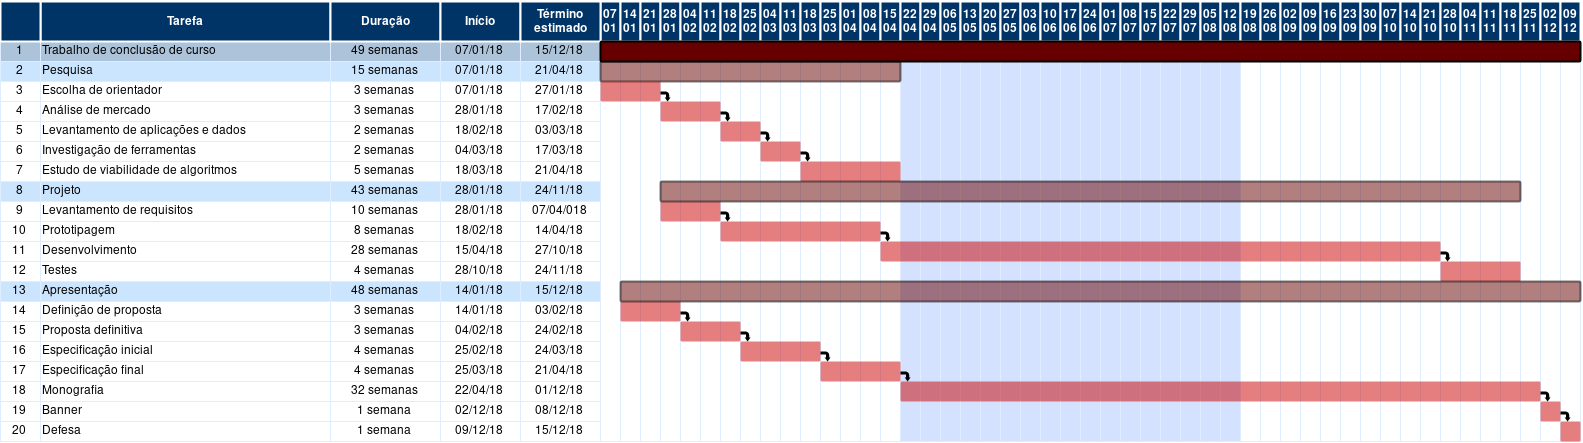
\includegraphics[width=6.5in]{imagens/diagrama_gantt}
    \caption{Diagrama de Gantt.}
    \label{fig:gantt}
\end{figure}

Desta forma, nos organizamos para realizar a implementação do sistema, separando
as tarefas a serem realizadas nas categorias: pesquisa, projeto, e apresentação.
Utilizamos o cronograma oficial da disciplina de TCC para elaborar um diagrama de Gantt na
Figura~\ref{fig:gantt} com a sequência de tarefas a serem divididas pelo grupo
ao longo do ano para cada semana. Indicamos também o período extra-escolar em
fundo azul, quando haverá desenvolvimento do sistema de forma mais lenta e
sem cronograma específico.

\chapter{Especificação de Requisitos do Sistema}

Tomando-se como base as tecnologias anteriormente citadas, definimos com mais
detalhe as necessidades do sistema para priorizar o trabalho descrito no
capítulo de \textbf{``Metodologia do Trabalho''}.

\begin{figure}[H]
    \centering
    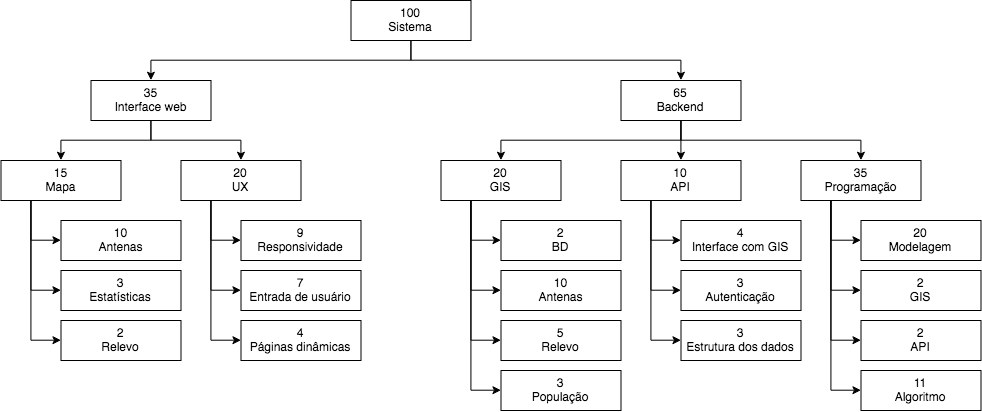
\includegraphics[width=6in]{imagens/arvore_prerequisitos}
    \caption{Árvore de pré-requisitos do sistema.}
    \label{fig:arvore_prerequisitos}
\end{figure}

Para definir os requisitos do nosso sistema, foi elaborada uma árvore de
pré-requisitos, listando a prioridade total dada a cada componente do sistema
final na Figura~\ref{fig:arvore_prerequisitos}. A divisão do trabalho será
feita nos componentes de \textit{front-end} e \textit{back-end}, como discorrido
anteriormente.

Como evidenciado pela figura~\ref{fig:arvore_prerequisitos}, a ênfase deste projeto será no \textit{back-end};
em especial, na parte de modelagem e programação relacionadas ao cálculo de
otimização da posição de antenas. As outras duas partes relevantes do
\textit{back-end} tratam, respectivamente, da instalação e uso do banco de dados do SIG, e
da comunicação externa de dados via API.

Embora tenha uma ênfase menor, o \textit{front-end} da interface web também será
um requisito fundamental de projeto, separado na experiência do usuário e na
visualização do mapa.

Definido o escopo, começamos a pensar, junto com nosso orientador, sobre os
requisitos do projeto. A estratégia utilizada foi o \textit{brainstorming}, leitura de
obras de referência na literatura de otimização de antenas, e pesquisa de softwares com escopo parecido.
A ideia inicial era ter como ator principal do sistema o funcionário cadastrado
de uma empresa de instalação de antenas, porém depois consideramos que seria
complementar ao projeto considerar um usuário não-comercial, assim
como um usuário administrador. Nessa fase, perguntamo-nos como o nosso projeto
poderia ajudar esses atores, qual informação ele deveria produzir. Esse processo
nos levou à modelagem de diversos casos de uso de interesse do sistema. Alguns
foram deixados de lado por fugirem ao escopo do MVP, e estão listados na seção
\textbf{``Perspectivas de Continuidade''} do último capítulo.

\section{Casos de Uso}

\newcounter{usecasecounter}
\newcommand{\usecase}[1]{\refstepcounter{usecasecounter}\label{usecase:#1}\arabic{usecasecounter}}

\subsection{Atores}
\begin{itemize}
\item Administrador
\item Funcionário cadastrado de Empresa de instalação de antenas
\item Usuário não-comercial
\end{itemize}

\subsection{Requisitos funcionais}
\begin{itemize}
\item Efetuar \textit{login}
\item Efetuar \textit{logout}
\item Cadastrar usuário no sistema
\item Exibir mapa com ERBs
\item Exibir mapa com cobertura celular estimada
\item Exibir localização ideal para instalação de uma nova ERB
\item Adicionar nova ERB
\item Fazer \textit{login} por OAuth2
\item Acessar API
\item Exibir ERBs às quais o celular do usuário está conectado
\item Exibir mapa com qualidade do sinal por operadora
\item Estimar geolocalização do usuário
\item Listar usuários
\end{itemize}

\subsection{Requisitos não-funcionais}
\begin{itemize}
\item Funcionalidades e código bem documentados
\item Interface acessível e simples
\item Ser responsivo
\item Ser dinâmico
\item Ser rápido
\item Ser seguro
\end{itemize}

\subsection{Descrição dos casos de uso}

\noindent \textbf{Caso de Uso \usecase{login}}: Efetuar \textit{login} no sistema. \\
\textbf{Descrição}: Este caso de uso descreve o processo de autenticação no sistema. \\
\textbf{Evento iniciador:} Usuário informa seu nome de usuário e senha. \\
\textbf{Atores:} Administrador, Funcionário ou Usuário não-comercial. \\
\textbf{Pré-condições:} Usuário na página de login. \\
\textbf{Sequência de Eventos:}
\begin{enumerate}
\item\label{step:login:enter-login} Usuário informa seu nome de usuário e sua senha.
\item\label{step:login:authenticate} Sistema autentica o usuário e senha.
\item Sistema exibe página inicial com opções correspondentes ao nível de privilégio do usuário.
\end{enumerate}
\textbf{Pós-condições:} Usuário logado no sistema. \\
\textbf{Extensões:}
\begin{enumerate}
\item Usuário ou senha estão incorretos: Sistema exibe mensagem de erro (passo \ref{step:login:authenticate}).
\item Login por OAuth2: Sistema recebe token de autenticação externa para o acesso (passo \ref{step:login:enter-login}).
\end{enumerate}
\textbf{Inclusões}: -{}- \\

\noindent \textbf{Caso de Uso \usecase{logout}}: Efetuar \textit{logout} no sistema. \\
\textbf{Descrição}: Este caso de uso descreve o processo de \textit{logout} no sistema. \\
\textbf{Evento iniciador}: Usuário clica no botão de \textit{logout}. \\
\textbf{Atores}: Administrador, Funcionário ou Usuário não-comercial. \\
\textbf{Pré-condições}: Usuário logado no sistema. \\
\textbf{Sequência de Eventos}:
\begin{enumerate}
\item Usuário clica no botão de \textit{logout}.
\item Sistema exibe página inicial para usuários não-logados.
\end{enumerate}
\textbf{Pós-condições}: Usuário deslogado do sistema. \\
\textbf{Extensões}: -{}- \\
\textbf{Inclusões}: -{}- \\

\noindent \textbf{Caso de Uso \usecase{show-map}}: Exibir mapa \\
\textbf{Descrição}: Este caso de uso descreve o processo de exibição de um mapa centrado na localização do usuário. \\
\textbf{Evento iniciador}: Usuário requisita exibição de mapa. \\
\textbf{Pré-condições}: Usuário logado no sistema. \\
\textbf{Sequência de Eventos}:
\begin{enumerate}
\item Usuário requisita exibição de mapa.
\item Sistema pede que o usuário permita acessar sua geolocalização.
\item Usuário permite que sistema acesse sua geolocalização.
\item\label{step:show-map:user-centered-map} Sistema mostra um mapa centrado no usuário.
\end{enumerate}
\textbf{Pós-condições}: Mapa com ERBs apresentado. \\
\textbf{Extensões}: Usuário não permite: Sistema mostra mapa centrado numa localização padrão. (passo \ref{step:show-map:user-centered-map}) \\
\textbf{Inclusões}: Busca de mapa no OpenStreetMap (passo \ref{step:show-map:user-centered-map}) \\

\noindent \textbf{Caso de Uso \usecase{show-map-bs}}: Exibir mapa com ERBs. \\
\textbf{Descrição}: Este caso de uso descreve a exibição das ERBs em um mapa. \\
\textbf{Evento iniciador}: Usuário clica na opção ``Mapa de ERBs''. \\
\textbf{Atores}: Administrador, Funcionário. \\
\textbf{Pré-condições}: Usuário logado no sistema. \\
\textbf{Sequência de Eventos}:
\begin{enumerate}
\item Usuário clica na opção ``Mapa de ERBs''.
\item\label{step:show-map-bs:show-map} Sistema exibe mapa com ERBs da região.
\end{enumerate}
\textbf{Pós-condições}: Mapa com ERBs apresentado. \\
\textbf{Extensões}: -{}- \\
\textbf{Inclusões}: Caso de uso \ref{usecase:show-map} ``Exibir mapa'' (passo \ref{step:show-map-bs:show-map}) \\

\noindent \textbf{Caso de Uso \usecase{show-map-location}}: Exibir mapa centrado em localização dada \\
\textbf{Descrição}: Este caso de uso descreve a exibição do mapa com ERBs
centrado em uma localização dada pelo usuário.  \\
\textbf{Evento iniciador}: Usuário insere a latitude e longitude e clica em ``Buscar''. \\
\textbf{Atores}: Administrador, Funcionário. \\
\textbf{Pré-condições}: Usuário logado no sistema e na página com mapa de ERBs. \\
\textbf{Sequência de Eventos}:
\begin{enumerate}
\item Usuário insere a latitude e longitude e clica em ``Buscar''.
\item\label{step:show-map-location:show-map} Sistema mostra o mapa de ERBs centrado na localização dada.
\end{enumerate}
\textbf{Pós-condições}: Mapa com ERBs centrado na localização dada apresentado. \\
\textbf{Extensões}: Latitude ou longitude inválida: Sistema mostra uma mensagem de erro (passo \ref{step:show-map-location:show-map}) \\
\textbf{Inclusões}:
\begin{enumerate}
\item Busca de mapa no OpenStreetMap (passo \ref{step:show-map-location:show-map})
\item Caso de uso \ref{usecase:show-map-bs} ``Exibir mapa com ERBs'' (pré-condição)
\end{enumerate}

\noindent \textbf{Caso de Uso \usecase{show-map-erb-operator}}: Exibir ERBs no mapa por operadora. \\
\textbf{Descrição}: Este caso de uso descreve a exibição do mapa com ERBs para
uma operadora definida pelo usuário. \\
\textbf{Evento iniciador}: Usuário seleciona uma operadora. \\
\textbf{Atores}: Administrador, Funcionário. \\
\textbf{Pré-condições}: Usuário logado no sistema e na página com mapa de ERBs. \\
\textbf{Sequência de Eventos}:
\begin{enumerate}
\item Usuário seleciona uma operadora.
\item Sistema mostra o mapa de ERBs da operadora dada pelo usuário.
\end{enumerate}
\textbf{Pós-condições}: Mapa com ERBs da operadora escolhida. \\
\textbf{Extensões}: -{}- \\
\textbf{Inclusões}: Caso de uso \ref{usecase:show-map-bs} ``Exibir mapa com ERBs'' (pré-condição) \\

\noindent \textbf{Caso de Uso \usecase{find-optimal-location}}: Encontrar local de instalação de ERBs.
\textbf{Descrição}: Este caso de uso descreve a exibição de posições otimizadas \\
para instalação de ERBs.
\textbf{Evento iniciador}: Usuário clica na opção ``Calcular posição para instalação''. \\
\textbf{Atores}: Administrador, Funcionário. \\
\textbf{Pré-condições}: Usuário logado no sistema e na página ``Mapa de ERBs''. \\
\textbf{Sequência de Eventos}:
\begin{enumerate}
\item Usuário clica na opção ``Calcular posição para instalação''.
\item Sistema exibe um formulário com campos: ``Quantidade de ERBs a serem
instaladas'' e ``Parâmetros a serem considerados no cálculo''.
\item Usuário preenche o formulário e clica em avançar.
\item Sistema solicita para o usuário selecionar a região de interesse.
\item Usuário seleciona a região de interesse.
\item Sistema informa que operação pode demorar alguns momentos.
\item\label{step:find-optimal-location:show-positions} Sistema indica os locais calculados no mapa.
\item Sistema mostra número de usuários atendidos por cada nova antena.
\end{enumerate}
\textbf{Pós-condições}: Mapa com posições otimizadas apresentadas. \\
\textbf{Extensões}: Operação demora muito tempo: Sistema informa que não foi
possível calcular a posição (passo \ref{step:find-optimal-location:show-positions}) \\
\textbf{Inclusões}: Caso de uso \ref{usecase:show-map-bs} ``Exibir mapa com ERBs'' (pré-condição). \\

\chapter{Projeto e Implementação}

Definidos os requisitos e as tecnologias a serem utilizadas, e os conceitos
abordados em cada algoritmo, iniciaram-se as implementações conforme o capítulo
\textbf{``Metodologia do Trabalho''}. As partes relevantes do sistema e as
soluções encontradas estão mencionadas abaixo.

\section{\textit{Back-end}}

A utilização do \textit{back-end} no sistema foi, no geral, para a obtenção de
dados existentes em banco e a computação de novas posições ótimas para as antenas.
Apesar de não estar diretamente visível ao usuário, esta parte do sistema se
mostrou também com dificuldades intrínsecas que nós precisamos enfrentar. Nas
seções a seguir, detalharemos as medidas tomadas em cada etapa.

\subsection{Modelos de ERBs}

Anteriormente, comentamos sobre a criação de dois modelos de ERBs, cada um
proveniente de uma dentre duas bases de dados. Uma base delas utiliza
dados oficiais da Anatel para indicar as antenas oficialmente registradas,
portanto que pertencem a uma única operadora legalmente~\cite{mapa-erb}.
Estas antenas foram denominadas ``Antenas Apropriadas'' (``\textit{Owned Base
Stations}''), pois indicam as operadoras às quais pertencem.

A outra base apresenta antenas distinguíveis por um identificador global,
portanto acaba exibindo uma única antena compartilhada como várias entradas do
banco de dados para cada respectiva operadora~\cite{opencellid}. Como possuem um
identificador de padrão global, estes dados foram chamados de ``Antenas
Identificadas'' (``\textit{Identified Base Stations}'') no código. Tanto os
dados dessa base quanto da anterior são representados como arquivos
\textit{Comma-Separated Values} (CSV) em suas origens.

Para cada modelo, criamos um \textit{script} que parseia os dados de entrada e
popula as entradas no banco de dados. Estes \textit{scripts} utilizaram o
suporte nativo do Django a utilitários da linha de comando para facilitar o
uso.

Os dados da Anatel foram extraídos e desestruturados em latitude e longitude,
operadora, Unidade Federativa (UF), município e endereço. Também foram criados
modelos adicionais para agregar antenas por operadora e por UF.

Para a base de dados aberta, foram utilizados como parâmetros a latitude e a
longitude, os campos do \textit{Cell Global Identity} (CGI), que identifica cada
antena, o tipo de rádio, e o sinal médio detectado. Como esta base possui dados
globais de antenas, filtramos apenas para os do Brasil; para isso, utilizamos
um dos campos do CGI, o \textit{Mobile Country Code} (MCC) -- que é único por
país --, como filtro das linhas do arquivo CSV. O MCC do Brasil é 724~\cite{mcc-mnc}.

Com estes dois scripts, conseguimos importar todos os dados relevantes destes
arquivos para o PostGIS. Porém, em etapas posteriores do projeto, foi necessário
escolher entre um modelo principal para implementar a solução. Para chegar a um
consenso, conversamos dentro do grupo, com o orientador e com Milton Kaoru
Kashiwakura, Diretor de Projetos Especiais e Desenvolvimento do NIC.br.

Devido à proeminência do compartilhamento de antenas entre empresas de
telecomunicação, optamos por utilizar a segunda base nas etapas subsequentes do
projeto como análise mais realista da cobertura celular no Brasil. Como não há
uma correlação direta das antenas com cada operadora ao contrário da outra
base, utilizou-se um campo específico do CGI, denominado \textit{Mobile Network
Code} (MNC) -- que especifica uma única operadora dentro de um país~\cite{mcc-mnc}
--, para verificar a qual empresa pertence cada antena nas etapas subsequentes
do trabalho. Assim, foi criado um modelo no banco de dados específico para
guardar os valores de MNC e respectivas operadoras, pois será útil para filtrar
estes dados.

\subsection{Modelagem}

% TODO Eric: Diagrama de modelos

\subsection{Clusterização}

Um dos principais desafios na implementação foi realizar a exibição de múltiplas
antenas como pontos em um mapa. Como muitas ERBs ficam próximas das outras e,
portanto, difíceis de serem visualizadas separadamente, utilizou-se um
\textit{plugin} próprio da biblioteca de mapa para a clusterização de pontos,
facilitando a identificação da quantidade de antenas em uma região, com exibição
variável com o zoom.

\begin{figure}[H]
    \centering
    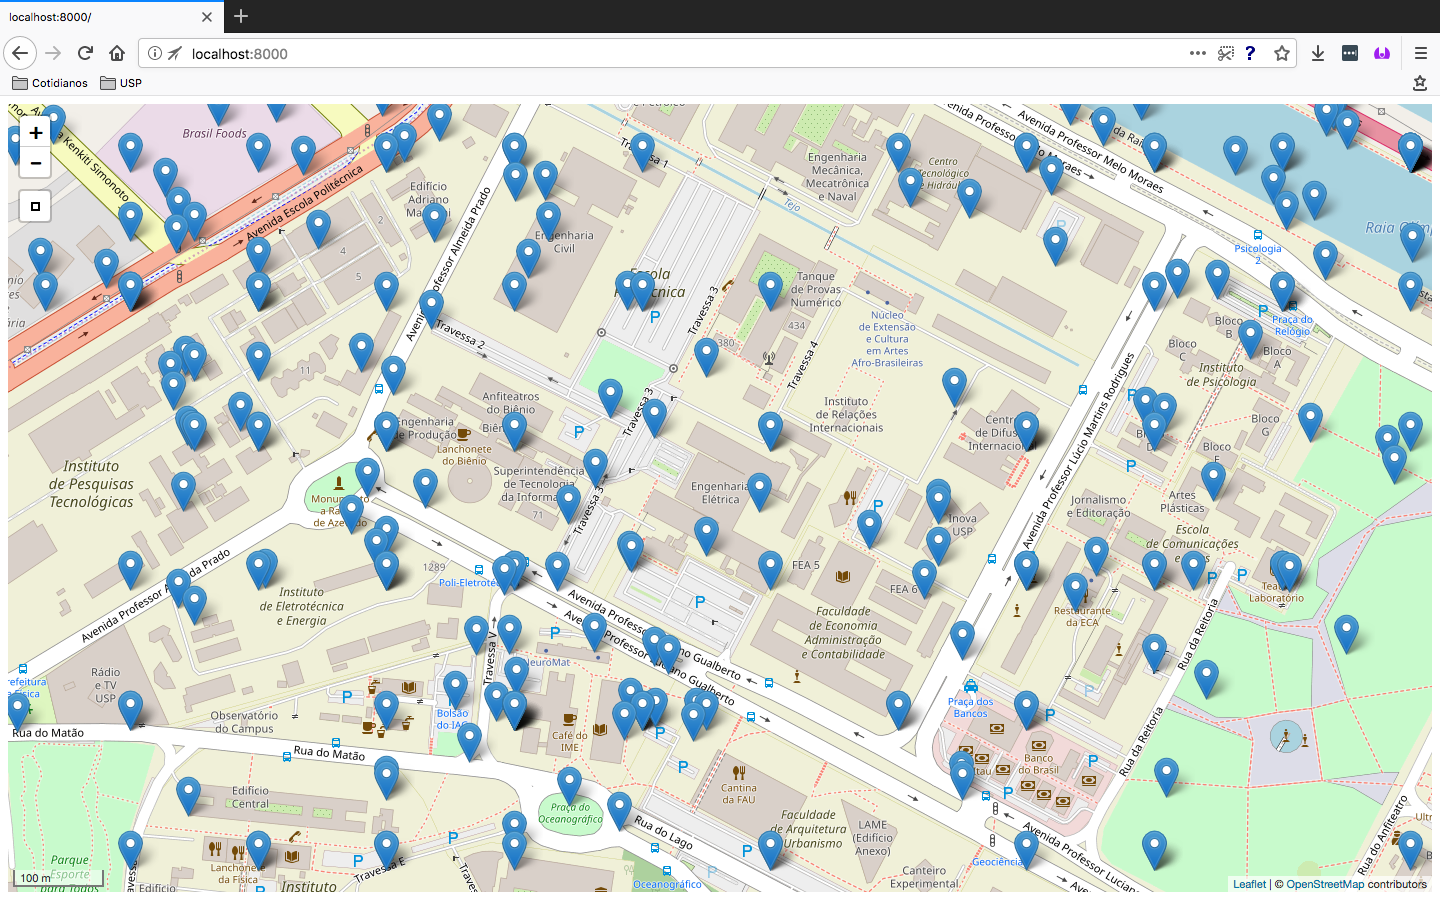
\includegraphics[width=6in]{imagens/mapa_sem_clusters}
    \caption{Mapa de ERBs sem clusterização.}
    \label{fig:mapa_sem_clusters}
\end{figure}

\begin{figure}[H]
    \centering
    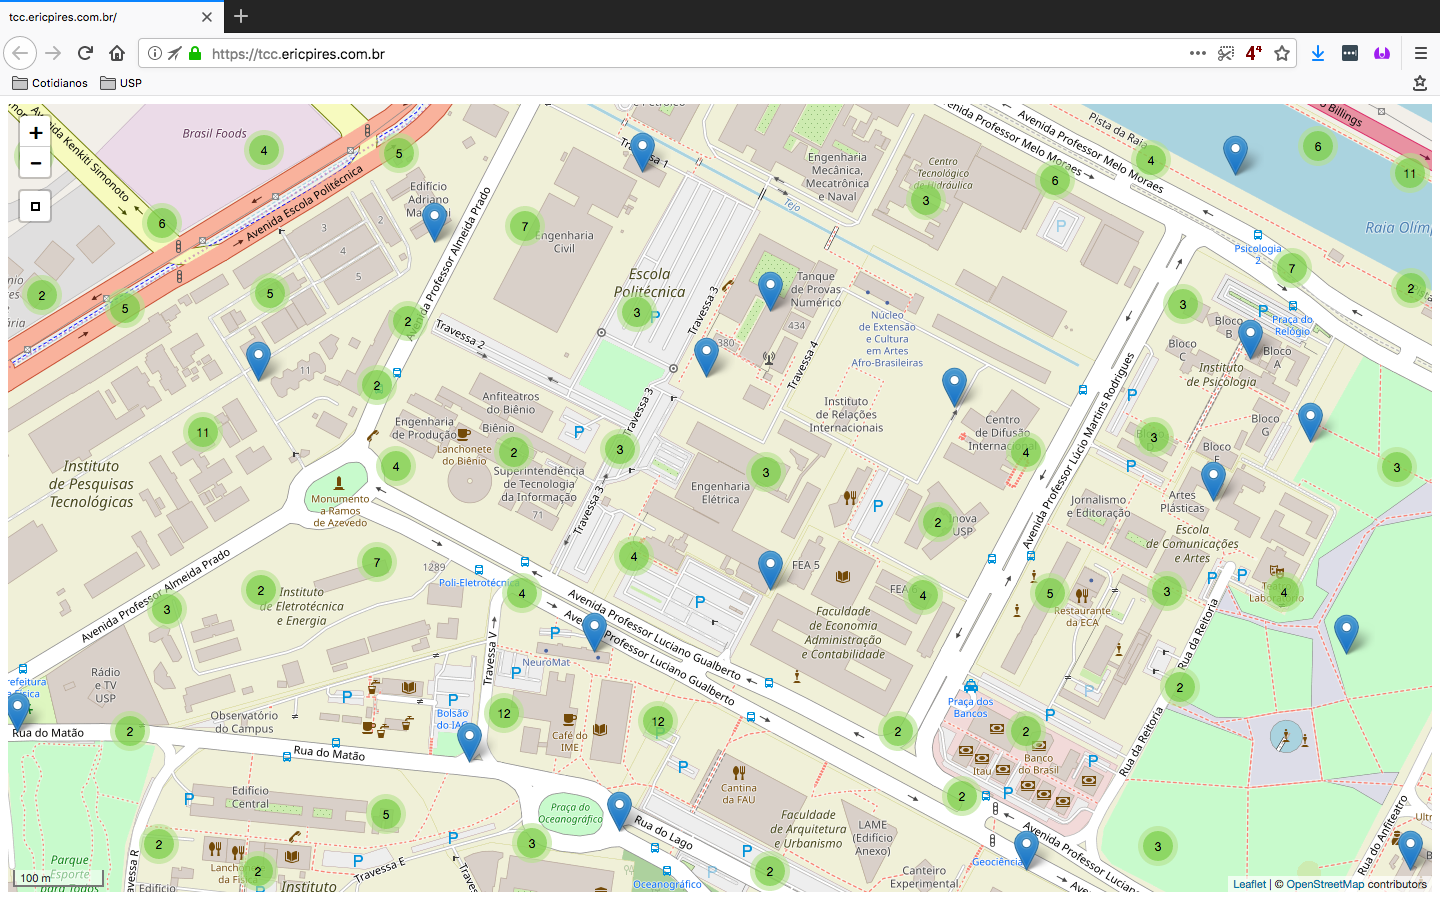
\includegraphics[width=6in]{imagens/mapa_com_clusters}
    \caption{Mapa de ERBs com clusterização.}
    \label{fig:mapa_com_clusters}
\end{figure}

Com o uso desse plugin, a exibição de até cerca de 500 antenas na tela tornou-se
possível. Porém, mais antenas do que isso causavam vários problemas relacionados
a uma grande quantidade de dados, como demora na transmissão por HTTP,
requisições intensivas ao servidor, e problemas de memória no navegador do
cliente. Algumas medidas foram tomadas tanto no \textit{back-end} quanto no \textit{front-end}
para tentar amenizar estes efeitos, como otimizar scripts mas sem gerar vantagens muito perceptíveis.

Dessa forma, resolveu-se utilizar algoritmos de clusterização no \textit{back-end}, e
então realizar a integração com o \textit{front-end}. A primeira tentativa envolveu a
utilização de uma biblioteca \textit{open-source} específica para o GeoDjango,
chamada ``\texttt{Anycluster}''~\cite{anycluster}. Embora tenha sido feita para uma
configuração de servidor similar à utilizada no projeto, a instalação e
documentação se mostraram confusas e incompletas. E mesmo com tentativas de
ajuste manual no código, incluindo refatoração das partes não-essenciais da
aplicação, não foi possível integrar este código à nossa base. Além disso,
a análise do código indica que não há nenhuma forma de
cache dos dados de clusterização, o que não resultaria em velocidades adequadas
para uma aplicação de visualização em mapa.

Procurou-se então uma segunda alternativa de clusterização, com implementação
própria para este projeto. A solução envolve utilizar o \textit{tiling} de grade que o
OpenStreetMap utiliza para carregar as imagens. A clusterização foi feita com
fórmulas do PostGIS específicas para clusterização de pontos. Para o cache dos
\textit{clusters}, utilizou o cache padrão do Django. Os resultados gerados pelo programa
eram corretos, mas o uso alto de memória e o tempo para clusterizar antes de
cache inviabilizam o uso no servidor. Foi realizado um aumento na capacidade
da máquina do host, mas não houve ganhos consideráveis. Além disso, os dados
de \textit{cluster} ficam com aparência estranha, onde a separação em grids fica muito
perceptível por não ser natural.

A terceira tentativa utilizou a mesma ideia anterior, porém para um dado nível
de zoom, seriam utilizados os \textit{clusters} para um zoom mais próximo do mapa,
portanto usando 4 vezes mais dados. Ainda houve alguns \textit{clusters} estranhos na
visualização em mapa, embora consideravelmente melhores no geral; mas combinado com o uso de
dados muito alto tanto em processamento quanto em rede, uma utilização com
muitos clientes se tornaria inviável.

Em seguida, na quarta tentativa, optamos por salvar os \textit{clusters} em banco de
dados, onde são indexados por zoom como nas tentativas anteriores. Para acelerar
o algoritmo de cálculo de \textit{clusters}, utiliza-se os \textit{clusters} de um zoom menor para
gerar os de zooms maiores. Foram feitas algumas iterações com diferentes funções
de clusterização do PostGIS para obter resultados melhores. A utilização de
modelos ao invés de cache resultou em uma fácil integração com o \textit{front-end} já
existente, dada a facilidade do Django para lidar com modelos na API. Porém,
os resultados obtidos foram inesperados, com clusters baseados na distância
ponto-a-ponto ao invés de ao redor de um centro de massa. Dessa forma, lugares
com muitas antenas lado-a-lado, em uma área com alta densidade de pontos como a
cidade de São Paulo, aparecem como um único \textit{cluster}, independentemente do zoom,
e às vezes muito longe do centro, deixando muits áreas vazias.

A quinta tentativa se baseou nas demais, e também no conceito de \textit{Geohash}
(anotação de cada região em um mapa com caracteres alfanuméricos, dividindo cada
região sucessiva do globo em 16 partes). Foi selecionada uma precisão (i.e. um
número de caracteres do \textit{geohash}) diferente para cada zoom, seguindo-se como
referência a biblioteca  ``\texttt{django-geohash-cluster}''~\cite{geohashcluster}, sendo
que a precisão máxima é de 7 caracteres, equivalente a uma precisão de aproximadamente 76
metros no Equador, o que é o suficiente para níveis de zoom.
Além disso, o código do \textit{front-end} foi modificado especificamente para fins de
performance, assim obtendo clusterizações com visualização mais natural.
Graças ao suporte do GeoDjango para inserir o geohash em queries, foi possível
realizar a implementação em um algoritmo simples, sem escrever as queries
manualmente. A principal desvantagem deste algoritmo foi a extrema demora para
realizar as clusterizações em comparação com os demais algoritmos; porém, o
resultado final com a integração de clusterização \textit{front-end} e \textit{back-end} foi
melhor em desempenho. Outra desvantagem foi que, como não há correspondência direta entre
níveis de zoom do mapa e precisões de \textit{geohash}, determinados níveis de zoom
demoram mais tempo para ler os dados. Além disso, há algumas pequenas falhas
visuais perto das bordas, que foram corrigidas posteriormente. Por fim,
foram realizadas alterações na API para tornar a transição entre \textit{clusters} e
ERBs na exibição do mapa opaca para o usuário final -- ou seja, o \textit{script} de exibição do mapa do
navegador enxerga um único \textit{endpoint} e não diferencia quando o servidor opta por
enviar dados de antenas ao invés de \textit{clusters} para zooms menores.

Este algoritmo foi expandido para também permitir a filtragem por operadora de
celular. Esta filtragem se baseia no campo MNC do identificador de cada estação
radiobase, que distingue a empresa responsável. Para filtros mais precisos, como
tipo de tecnologia celular, não será utilizada clusterização, com carregamento e
exibição diretamente no mapa -- já que inclui um número menor de antenas a serem
exibidas, e varia com o caso de uso de cada usuário, portanto sendo um processo
menos repetitivo para o servidor que não se beneficia de mecanismo de cache.

Vale notar que, para a implementação de filtragem por operadora, os \textit{clusters}
de todas as antenas utilizam um campo nulo para representar a operadora. Isso é
importante porque, ao exibir os \textit{clusters} sem filtro específico de operadora, na
realidade, deverá ser feito filtro por operadora igual ao valor nulo. Esta
distinção terá maior importância quando o cliente requisitar dados de clusters
pela API, como descrito mais adiante.

\subsection{Métodos Numéricos}

Em um primeiro momento, utilizamos três métodos para comparação entre
algoritmos: Taguchi, Basinhopping e SQSQP. A função de otimização foi
desacoplada da implementação do método numérico. Desse modo, podemos combinar
quaisquer métodos numéricos implementados com quaisquer funções de otimização.

Para os métodos Basinhopping e SQSQP, usamos a implementação disponível na
biblioteca ``\texttt{scipy}''~\cite{scipy}.

Já o método Taguchi foi implementado de acordo com a especificação especificada
no capítulo \textbf{``Aspectos Conceituais''}. Os arrays ortogonais usados pelo
método foram implementados como uma tabela, uma vez que seu cálculo é uma
operação complexa, e os casos de uso preveem o uso de poucos parâmetros no
método Taguchi. Usamos a biblioteca ``\texttt{numpy}''~\cite{numpy} para as operações com
\textit{array}, uma vez que ela provê operações eficientes nessas estruturas de dados.

Por fim, escolhemos o Método Taguchi, pois ele se comportou melhor que os demais
nos testes, encontrando mais mínimos globais que o SQSQP e o Basinhopping.
Além disso, temos um entendimento melhor de seu funcionamento uma vez que nós
que o implementamos. Os detalhes sobre os testes mencionados
encontram-se no capítulo Testes e Avaliação.


\subsection{Interface de Programação de Aplicações}

A integração do \textit{back-end} com o \textit{front-end} foi feita feita por uma API HTTP, que
abstrai os dados e as funcionalidades necessários para a realização dos casos de
uso. Resumidamente, ela deverá ser responsável por três tarefas específicas:

\begin{itemize}
\item Realizar \textit{login} de usuários no sistema.
\item Exibir dados de mapas na tela.
\item Gerar otimização de posição de antena.
\end{itemize}

Desta forma, foram expostos \textit{endpoints} para cada uma das tarefas. A utilização
da biblioteca Django REST Framework facilitou o processo de integração da API
ao \textit{back-end} desenvolvido. O cliente de \textit{front-end} -- no caso, o Vue -- poderá descobrir
estes \textit{endpoints} a partir de um outro \textit{endpoint} específico que expõe estas informações,
de forma a tornar refatorações do \textit{back-end} dinâmicas.

Algumas alterações tiveram que ser feitas tanto na configuração do Django quanto
na criação de \textit{endpoints} de API para a realização esperada dos casos de uso. A primeira
se refere ao \textit{login} de usuários, pois necessitou de reconfiguração da
autenticação do Django. Esta autenticação foi modificada para permitir que, por
um \textit{endpoint} específico de \textit{login}, um usuário realize uma requisição POST com seu
nome de usuário e senha e receba um \textit{token}, que pode ser utilizado nas requisições
autenticadas subsequentes. Como a autenticação padrão do Django não utiliza
\textit{tokens}, mas sim parâmetros de sessão específicos, alteramos esta configuração.

Outra modificação se refere à exibição de dados no mapa. Devido ao esquema de
clusterização por \textit{geohash} descrito anteriormente, optou-se por uma abordagem
opaca na API, aonde o usuário deverá indicar apenas as coordenadas da tela, o
tamanho de zoom atual, e o filtro de operadora. Dessa forma, foi descrita
lógica adicional neste \textit{endpoint} para converter o tamanho de zoom à precisão de
geohash correspondente. Além disso, o filtro de operadora foi complementado com
o caso geral de não filtrar por operadora, pois a modelagem dos \textit{clusters} no
banco de dados requer um filtro específico para \textit{clusters} sem filtro de
operadora.

\subsection{Bancos de Dados Externos}

Alguns dados adicionais mencionados anteriormente, que não serão persistidos no
banco de dados, são referentes a população e relevo. Ao longo de nossa pesquisa,
nos foi indicado o uso da Google Earth Engine\cite{earthengine}, que é uma plataforma
de dados geoespaciais disponível publicamente para ferramentas de análise
científica e pesquisa. Dentro desta plataforma, dois \textit{datasets} estudados para uso no sistema
são ``\texttt{USGS/SRTMGL1\_003}'' para topografia, e ``\texttt{WorldPop/POP}''
para densidade populacional.

O Google Earth Engine possui uma API oficial em Python, que foi estudada e
implementada no \textit{back-end}. A implementação criada permite persistir dados no
cache do servidor, para evitar que valores frequentemente utilizados nos
algoritmos de otimização (i.e. uma única área analisada repetidamente) sejam baixadas
novamente a cada execução.

\subsection{Instalação de Servidor}

O \textit{back-end} do sistema foi instalado em um servidor remoto para
apresentações e testes. Utilizou-se o serviço DigitalOcean para a virtualização
de servidor, onde subiu-se a instância por SSH em uma distribuição Ubuntu. As
chaves SSH foram distribuídas aos integrantes do grupo e ao orientador para
permitir o acesso. Nesta máquina, instalamos o repositório em Python, o banco
de dados PostgreSQL, e as aplicações adicionais necessárias para o
GeoDjango/PostGIS. Os passos tomados na configuração a seguir foram, fora de
ordem:

\begin{itemize}
\item Criar e ativar um ambiente virtual do Python (\texttt{virtualenv}).
\item Instalar dependências em Python do projeto.
\item Obter a extensão do PostGIS, e as bibliotecas GEOS, PROJ.4, GDAL, GeoIP2.
\item Criar um \textit{schema} no banco de dados para a aplicação.
\item Carregar dados de antenas apropriadas e identificadas.
\item Gerar diretório de arquivos estáticos do Django.
\item Obter arquivos de localização via IP da biblioteca GeoIP2.
\item Registrar-se no Google Earth Engine, gerar \textit{token} de autenticação,
e salvar no ambiente de usuário.
\item Criar usuários administradores para os membros do grupo e para
demonstração.
\item Habilitar cache em disco por banco de dados.
\end{itemize}

Estes passos foram reproduzidos em um \texttt{README} do repositório, para
facilitar a criação de novos ambientes de desenvolvimento.

Ainda neste servidor virtual, foram instalados o Nginx e o Gunicorn, para o
\textit{proxy} e o acesso HTTP, respectivamente. Também foi utilizado um nome de
domínio para o servidor, que foi configurado no Nginx. Além disso, por questão
de segurança, também configurou-se o acesso HTTPS ao servidor, através do Let's
Encrypt e sua configuração para \textit{proxy}.

Por fim, para facilitar o deployment da aplicação para testes, configurou-se
o repositório local do Git como um repositório remoto, permitindo que seja
atualizado por SSH com um único comando; e as regras de \textit{pull} do
repositório foram modificadas para aplicar novas alterações no código
instantaneamente -- como migração de banco de dados, coleta de arquivos
estáticos, novos \textit{endpoints}, dentre outros.

Uma medida tomada por segurança e por limitações técnicas na instalação do
\textit{back-end} foi a utilização de ambientes de desenvolvimento -- isto é,
a definição manual de variáveis do Django, sensíveis e/ou específicas por
máquina. Para isto, foi criado um novo arquivo, \texttt{config\_settings.py},
que é importado pelo arquivo de configurações padrão do Django
(\texttt{settings.py}) e é ignorado pela ferramenta Git. Dentre as variáveis
deste arquivo, estão:

\begin{itemize}
\item Uma \textit{flag} de debug, utilizada pelo Django para exibir informações
sensíveis de erro quando habilitada.
\item Uma chave secreta, utilizada para gerar \textit{hashes} de segurança.
\item Lista de \textit{hostnames} aceitos para conexões de entrada, que foi
definida para os IPs da máquina e o nome de domínio.
\item A conexão ao banco de dados, com usuário, senha e \textit{schema}.
\item Dados de acesso a autenticação social em serviços como GitHub e Facebook.
\end{itemize}

Alguns dados e parâmetros acima foram colocados como opcionais, para facilitar a
instalação de ambientes de desenvolvimento. Por exemplo, a biblioteca GeoIP2,
que tenta estimar a localização do usuário pelo IP, foi colocada no código como
dependência opcional, devido ao tamanho dos arquivos consumidos e à falta de
necessidade de testes para uso. Os dados de acesso para serviços sociais também
foram tornados opcionais por razões semelhantes.

\section{\textit{Front-end}}
Para elaborar o \textit{front-end}, usamos o \textit{framework} Vue.js.
O front-end da nossa aplicação foi responsável pela parte visual, pela
comunicação do cliente com a API em Django, pela exibição dos dados no mapa,
e pelo recebimento das entradas do usuário. Nas seções a seguir, detalharemos
como planejamos e implementamos o cada uma dessas partes.

\subsection{Projeto de Telas}
O planejamento do \textit{front-end} começou com o desenho das telas. Pensamos em telas
que implementassem os casos de uso, além de serem fáceis de usar tanto em \textit{desktop}
como em \textit{smartphones}.

A primeira tela projetada foi a tela de mapas. Inicialmente,
ela teria o mapa com os clusters e um menu lateral com opções de filtro por
operadora e tecnologia, opções de remoção, adição e exportação de ERBs e um
botão para executar o algoritmo de posição ideal a partir de parâmetros fornecidos
pelo usuário. Criamos os desenhos com papel e lápis, visto que tratam-se de uma
representação de baixa fidelidade.

\begin{figure}[H]
    \centering
    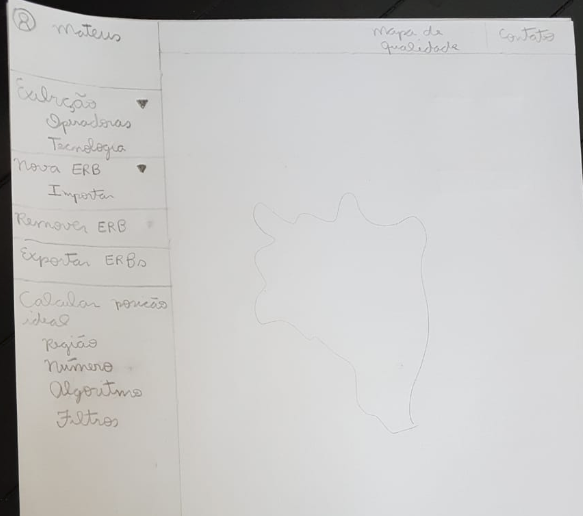
\includegraphics[width=4in]{imagens/rascunho-mapa}
    \caption{Projeto inicial da tela de mapas.}
    \label{fig:rascunho_mapa}
\end{figure}

Depois de algumas iterações, removemos algumas funcionalidades e adicionamos
outros filtros.

Outra tela projetada foi a tela inicial, com imagens do sistema
funcionando, textos explicativos e um formulário de contato. O objetivo dessa tela
é fornecer uma ideia inicial das \textit{features} do nosso projeto.

\begin{figure}[H]
    \centering
    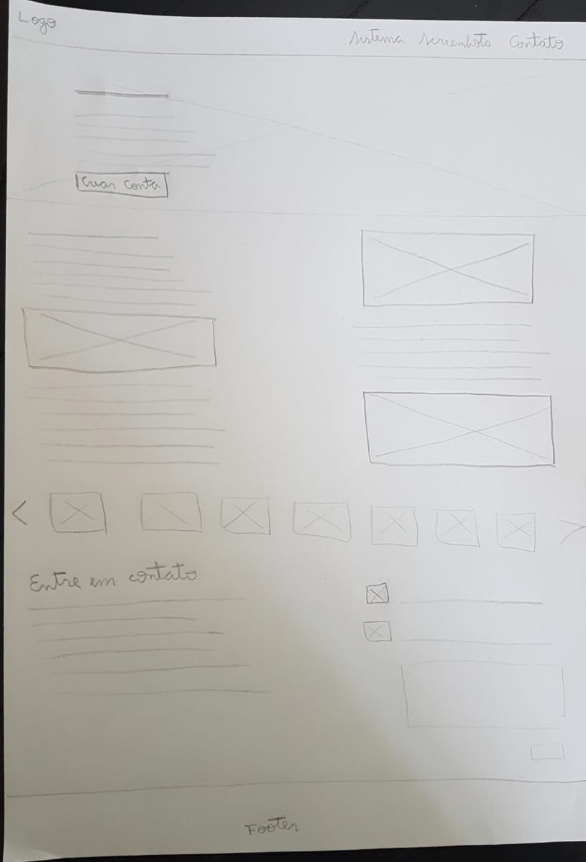
\includegraphics[width=4in]{imagens/rascunho-landing}
    \caption{Projeto inicial da tela inicial.}
    \label{fig:rascunho_landing}
\end{figure}

Pensamos também na tela de \textit{login}, na qual o usuário entra com seu nome de usuário e
senha. Essa seria a tela à qual ele seria redirecionado caso não estivesse logado.

\begin{figure}[H]
    \centering
    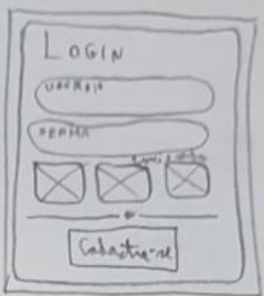
\includegraphics[width=2in]{imagens/rascunho-login}
    \caption{Projeto inicial da tela de login.}
    \label{fig:rascunho_login}
\end{figure}

\subsection{Implementação com Vue.js e Vuetify}
Usamos o \textit{framework} Vue.js no front-end do nosso projeto. Ele é um dos
\textit{frameworks} JavaScript mais populares da atualidade. Seu uso aumenta
muito a produtividade e organização do código, porque ele divide o sistema em
componentes pequenos e reusáveis. Outro benefício é o \textit{single page application} que o Vue.js viabiliza.
Com o \textit{single page application}, quando o usuário muda de tela, a página não é recarregada, apenas os
componentes diferentes que são trocados. Dessa forma, os componentes comuns a várias telas (como \textit{header} e \textit{footer})
nunca são recarregados. Isso propicia uma experiência mais fluida para o usuário.

Para tratar do visual do sistema, usamos a biblioteca Vuetify. Ela provê componentes
com visual característico do Material Design para o Vue.js. O Material Design é
uma linguagem visual criada pela Google que oferece um visual intuitivo que
se aproxima do design do mundo real com tinta e papel, trabalhando com camadas
e sombras que dão uma sensação tátil para o usuário. O uso do Vuetify facilitou
muito o desenvolvimento, pois não precisamos nos preocupar muito com o estilo de
cada elemento HTML.

Com relação às telas criadas, a tela de mapas usa um menu lateral, com opções de
filtro, um botão para executar o algoritmo de otimização, e um botão para exibir mapa de
calor. As opções de menu são seleções retangulares, por círculo, tecnologia e
cidades. Os filtros não implementados foram desabilitados.
Com isso, a tela final ficou pouco diferente da planejada na etapa de projeto de
telas.

\begin{figure}[H]
    \centering
    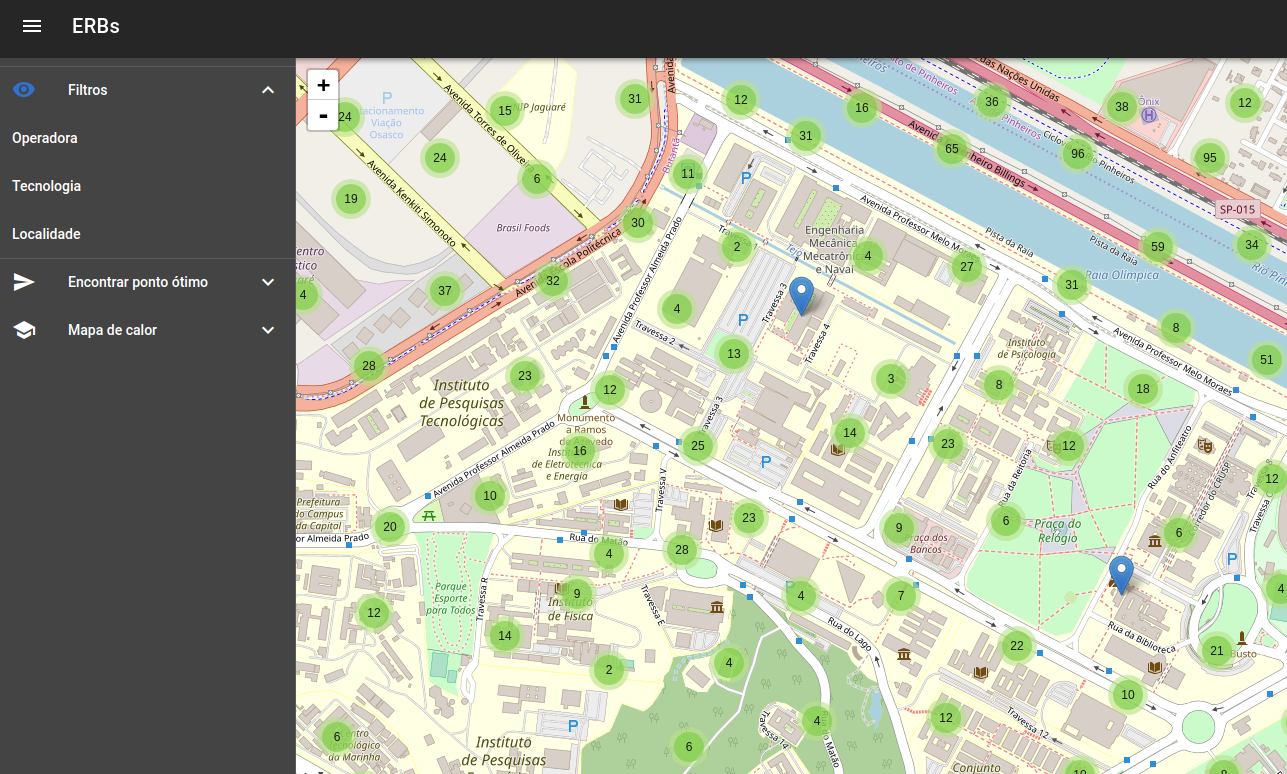
\includegraphics[width=6in]{imagens/tela-mapas}
    \caption{Tela de mapas.}
    \label{fig:tela_mapas}
\end{figure}

Ao escolher a opção de menu de seleção, podemos selecionar um retângulo ou
circunferência no mapa.

\begin{figure}[H]
    \centering
    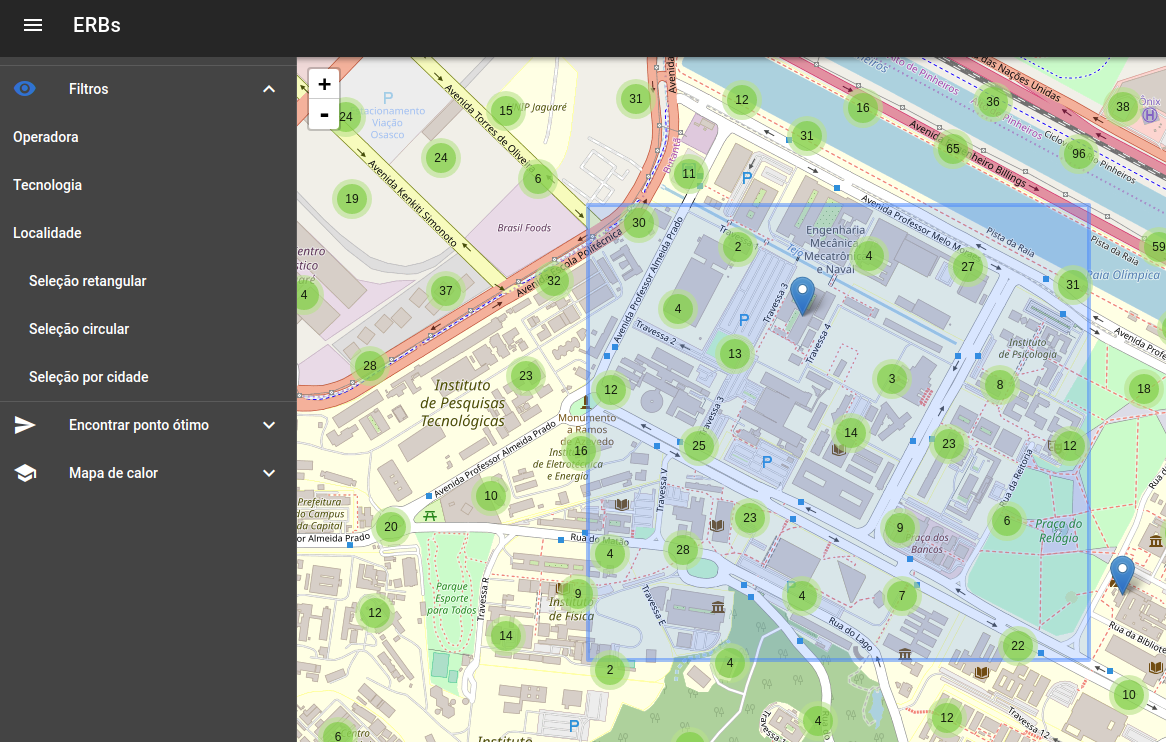
\includegraphics[width=6in]{imagens/tela-mapas-retangulo}
    \caption{Tela de mapas de seleção de área retangular.}
    \label{fig:tela_mapas_retangulo}
\end{figure}

A tela de \textit{login} foi um formulário simples com um campo de usuário e senha.

\begin{figure}[H]
    \centering
    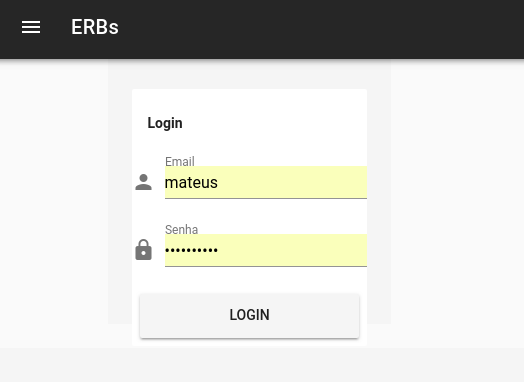
\includegraphics[width=4in]{imagens/tela-login}
    \caption{Tela de login.}
    \label{fig:tela_login}
\end{figure}
\subsection{Integração com \textit{Back-end}}

O \textit{front-end} foi responsável por fazer as chamadas de API.
Usamos o axios.js, uma biblioteca JavaScript bastante popular usada para fazer
requisições HTTP. Com ele, os retornos da API são convertidos
automaticamente em JSON, formato adequado para manipulação dentro do JavaScript.

Para a autenticação, na página de \textit{login}, enviamos o usuário e a senha digitados
pelo usuário para o \textit{endpoint} de \textit{login}. Caso válidos, o \textit{back-end} retorna um
\textit{token} necessário para realizar outras consultas. Usamos o gerenciador de estado Vuex
para armazenar esse token no escopo global. O Vuex permite que todos os
componentes da aplicação compartilhem o mesmo estado e que a mudança de estado
seja previsível e reflita para todos os componentes.

Possuindo esse \textit{token}, podemos fazer as chamadas de API restritas aos usuários
autenticados, e assim implementar nossos casos de uso. Isso foi feito adicionando-o
ao cabeçalho \texttt{Authorization} do HTTP. Caso o usuário tentasse acessar a
página de mapas e o \textit{token} não estivesse salvo no Vuex, o usuário seria
redirecionado à página de login.

% TODO: Uso da API, deployment do front-end

\chapter{Testes e Avaliação}

% TODO: Introdução do capítulo

\section{Testes de Métodos Numéricos}
Realizamos testes para verificar a corretude dos métodos numéricos que usamos, 
o SLSQP, o Basinhopping e o Taguchi. Usamos funções de teste para otimização
com mínimo global conhecido, e verificamos se era
igual à saída do método numérico. A seguir estão os testes do método Basinhopping.
A definição das funções e o domínio de busca está disponível na referência~\cite{optimization-functions}.
As linhas marcadas em cinza mostram funções na qual o método numérico não achou o mínimo global.

\begin{table}[H]
\begin{tabular}{l|l|l}
 Nome da função & Mínimo calculado & Mínimo global \\ \hline
\rowcolor{Gray}
Easom  &  f(100.0,100.0)=-0.0  &  f(3.14,3.14)=-1.0 \\
Himmelblaus  &  f(-3.78,-3.28)=0.0  &  f(3,2)=0 \\
Matyas  &  f(-0.0,-0.0)=0.0  &  f(0,0)=0.0 \\
\rowcolor{Gray}
Mccormick  &  f(2.59,1.59)=1.23  &  f(-0.55,-1.55)=-1.91 \\
\rowcolor{Gray}
Schaffer4  &  f(98.73,98.64)=0.5  &  f(0,1.25)=0.29 \\
Three hump camel  &  f(-0.0,-0.0)=0.0  &  f(0,0)=0.0 \\
\end{tabular}
\end{table}

A seguir estão os testes do método SLSQP.
\begin{table}[H]
\begin{tabular}{l|l|l}
 Nome da função & Mínimo calculado & Mínimo global \\ \hline
\rowcolor{Gray}
Easom  &  f(100.0,100.0)=-0.0  &  f(3.14,3.14)=-1.0 \\
\rowcolor{Gray}
Himmelblaus  &  f(-2.85,3.08)=0.17  &  f(3,2)=0 \\
\rowcolor{Gray}
Matyas  &  f(-0.65,-0.65)=0.02  &  f(0,0)=0.0 \\
\rowcolor{Gray}
Mccormick  &  f(2.51,1.51)=1.24  &  f(-0.55,-1.55)=-1.91 \\
\rowcolor{Gray}
Schaffer4  &  f(100.0,100.0)=0.5  &  f(0,1.25)=0.29 \\
Three hump camel  &  f(0.0,-0.0)=0.0  &  f(0,0)=0.0 \\
\end{tabular}
\end{table}

A seguir estão os testes do método Taguchi.
\begin{table}[H]
\begin{tabular}{l|l|l}
Nome da função & Mínimo calculado & Mínimo global \\ \hline
Easom  &  f(3.14,3.14)=-1.0  &  f(3.14,3.14)=-1.0 \\
Himmelblaus  &  f(3.0,2.0)=0.0  &  f(3,2)=0 \\
Matyas  &  f(0.0,0.0)=0.0  &  f(0,0)=0.0 \\
Mccormick  &  f(-0.55,-1.55)=-1.91  &  f(-0.55,-1.55)=-1.91 \\
\rowcolor{Gray}
Schaffer4  &  f(-98.51,-98.51)=0.5  &  f(0,1.25)=0.29 \\
Three hump camel  &  f(0.0,0.0)=0.0  &  f(0,0)=0.0 \\
\end{tabular}
\end{table}

% TODO

\section{Resultados}

% TODO

As fontes do trabalho foram disponibilizadas como código aberto no GitHub, e
foram separadas em dois repositórios: um para o \textit{back-end} Django, com
instruções de instalação para desenvolvimento local~\cite{repo-django}; e um
para o \textit{framework} de \textit{front-end} escrito em Vue~\cite{repo-vue}.
Além disso, esta monografia em si também está disponível no GitHub~\cite{repo-tcc}.

\chapter{Considerações Finais}

% TODO: Recapitulação e visão geral sobre o projeto

\section{Conclusões do Projeto de Formatura}

% TODO: Falar mais especificamente sobre o que deu certo e errado

\section{Contribuições}

% TODO Eric: Expressar as contribuições do TCC para o meio acadêmico, para a
% sociedade e para o grupo

\section{Perspectivas de Continuidade}

Ao longo da especificação de requisitos e da implementação, alguns aspectos
foram deixados de lado por fugirem do escopo do MVP. Porém, eles serão
interessantes em um produto final, agregando funcionalidades desejáveis aos
\textit{stakeholders}. Além disso, também será interessante detalhar o processo de
criação de empresa para a distribuição do produto.

\subsection{Plano de Negócio}

Também foi feito um estudo de implementação do projeto do MVP na concepção de
um produto real; em outras palavras, as etapas para prosseguir com a criação
de uma \textit{startup}. Em especial na própria Escola Politécnica, há uma
organização específica para promoção dessa cultura, chamada Núcleo de
Empreendedorismo da USP (NEU), que fomenta e dá suporte à criação de pequenas
empresas de alunos~\cite{neu}.

Em linhas gerais, estabelecemos um processo de implantação da empresa após a
conclusão do TCC, seguindo-se as recomendações do próprio NEU:

\begin{enumerate}
\item Entrar em contato com o NEU e avaliar recursos disponíveis no seu
programa de pré-aceleração, como contatos do mercado e mentoria de
empreendedorismo.
\item\label{business-landing-page} Completar a \textit{landing page} com os
principais pontos fortes do produto, e divulgar para os \textit{stakeholders}.
Assim, será possível obter \textit{feedback} sobre o interesse do mercado --
pelo número de acessos à página e pelo preenchimento de formulários de
notificações por e-mail --, além de estabelecer uma base de clientes realmente
interessada no negócio.
\item Utilizando-se como base o conceito de \textit{Business Model Canvas},
elaborar um modelo de negócio, listando os objetivos e medidas a serem tomados.
A princípio, seria dada ênfase na escolha de parceiros e clientes, com foco
secundário nas atividades e recursos da empresa.
\item Validar MVP com os primeiros usuários do sistema selecionados no passo
\ref{business-landing-page}. Com isso, será possível obter \textit{feedback} e
métricas de uso, estabelecidas de acordo com as seguintes hipóteses (baseadas
nos nossos recursos não-funcionais):
\begin{itemize}
\item O produto é de fácil utilização.
\item O sistema é útil para os instaladores de antenas.
\item Os clientes possuem confiança na qualidade do produto.
\end{itemize}
\item Com os dados coletados acima, aperfeiçoar o produto incrementalmente, em
preparação para reorganizar a estrutura da empresa. Isso permite aumentar o
número de clientes e a própria empresa em contrapartida, seguindo-se a ajuda
do NEU nesta etapa.
\end{enumerate}

Desta forma, podemos estabelecer a \textit{startup} de maneira adequada ao
mercado e voltada a resultados positivos, tanto na valorização do produto quanto
ao amadurecimento da empresa no ecossistema de empreendedorismo.

\subsection{Dados}

Da parte técnica do projeto, mais duas bases de dados que foram estudadas para
uso foram: a G-Econ~\cite{gecon}, da Universidade de Yale, que apresenta os dados de paridade de
poder de compra geograficamente; e o SIMET-NIC~\cite{simet}, com o acesso e
qualidade da Internet no Brasil. Estas duas bases de dados, em conjunto com as
anteriores, podem permitir uma análise aprofundada de parâmetros ótimos para a
instalação de novas antenas e avaliação da estrutura pré-existente; porém,
a relação destes dados não cabe ao nosso caso de uso principal desta monografia. Elas podem
ser úteis em uma análise futura, ao trabalhar em conjunto com os
\textit{stakeholders} para análises de instalação levando-se em conta parâmetros socioeconômicos,
que seriam mais interessantes a uma empresa de telecomunicação.

\subsection{Descrição dos Casos de Uso Adicionais}

Os casos de uso a seguir foram elaborados na etapa de ``Especificação de
Requisitos do Sistema'', porém foram deixados para uma implementação futura, já
que não afetam a demonstração do MVP.

\noindent \textbf{Caso de Uso \usecase{sign-up}}: Cadastrar usuário no sistema.  \\
\textbf{Descrição}: Este caso de uso descreve o cadastro de usuários no sistema \\
\textbf{Evento iniciador}: Usuário clica no botão ``Cadastrar usuário''. \\
\textbf{Atores}: Administrador, Funcionário ou Usuário não-comercial. \\
\textbf{Pré-condições}: Usuário não logado no sistema. \\
\textbf{Sequência de Eventos}:
\begin{enumerate}
\item Usuário clica no botão ``Cadastrar usuário''.
\item Sistema exibe página de cadastro.
\item Usuário digita nome, e-mail, senha e confirmação de senha.
\item\label{step:sign-up:send-email} Sistema valida dados e envia e-mail de confirmação para usuário.
\end{enumerate}
\textbf{Pós-condições}: Usuário cadastrado no sistema com confirmação de e-mail pendente. \\
\textbf{Extensões}:
\begin{enumerate}
\item Usuário já cadastrado: Sistema exibe mensagem de erro (passo \ref{step:sign-up:send-email})
\item Senha não é igual a confirmação de senha: Sistema exibe mensagem de erro (passo \ref{step:sign-up:send-email})
\end{enumerate}
\textbf{Inclusões}: Buscar usuário (passo \ref{step:sign-up:send-email}) \\

\noindent \textbf{Caso de Uso \usecase{confirm-email}}: Confirmação de e-mail. \\
\textbf{Descrição}: Este caso de uso descreve o processo de confirmação de um e-mail. \\
\textbf{Evento iniciador}: Usuário acessa a URL correspondente à confirmação de seu e-mail. \\
\textbf{Atores}: Administrador, Funcionário ou Usuário não-comercial. \\
\textbf{Pré-condições}: Usuário cadastrado no sistema com e-mail não confirmado. \\
\textbf{Sequência de Eventos}:
\begin{enumerate}
\item Usuário acessa a URL correspondente à confirmação de seu e-mail.
\item\label{step:confirm-email:validate-email} Sistema confirma a validade do e-mail do usuário.
\item Sistema redireciona o usuário para página inicial.
\end{enumerate}
\textbf{Extensões}: URL de confirmação inválida: Sistema mostra uma mensagem de
erro e redireciona o usuário para a página de \textit{login} (passo \ref{step:confirm-email:validate-email}). \\
\textbf{Inclusões}: -{}- \\

\noindent \textbf{Caso de Uso \usecase{add-bs}}: Adicionar nova ERB \\
\textbf{Descrição}: Este caso de uso descreve o processo de adição de novas
ERBs na base de dados. \\
\textbf{Evento iniciador}: Usuário clica na opção ``Adicionar ERB''. \\
\textbf{Atores}: Administrador, Funcionário. \\
\textbf{Pré-condições}: Usuário logado no sistema. \\
\textbf{Sequência de Eventos}:
\begin{enumerate}
\item Usuário clica na opção ``Adicionar ERB'' e clica em um ponto no mapa.
\item Sistema exibe formulário com dados a serem cadastrados sobre a nova ERB.
\item Usuário preenche formulário e clica em ``Salvar''.
\item\label{step:add-bs:save-bs} Sistema salva nova ERB.
\item\label{step:add-bs:show-map} Sistema exibe mapa com ERBs.
\end{enumerate}
\textbf{Pós-condições}: Mapa com ERBs apresentado e nova ERB salva na base de
dados. \\
\textbf{Extensões}: Dados inválidos: Sistema exibe mensagem de erro e exibe
formulário novamente (passo \ref{step:add-bs:save-bs}). \\
\textbf{Inclusões}: Caso de uso \ref{usecase:show-map-bs} ``Exibir mapa com ERBs'' (pré-condição e passo \ref{step:add-bs:show-map}).\\

\noindent \textbf{Caso de Uso \usecase{remove-bs}}: Remover ERB \\
\textbf{Descrição}: Este caso de uso descreve o processo de remoção de uma ERB da
base de dados. \\
\textbf{Evento iniciador}: Usuário clica na opção ``Remover ERB''. \\
\textbf{Atores}: Administrador, Funcionário. \\
\textbf{Pré-condições}: Usuário logado no sistema. \\
\textbf{Sequência de Eventos}:
\begin{enumerate}
\item Usuário clica na opção ``Remover ERB'' e seleciona uma ERB no mapa.
\item Sistema pergunta se usuário realmente deseja remover ERB.
\item Usuário responde ``Sim''.
\item Sistema remove ERB.
\item\label{step:remove-bs:show-map} Sistema exibe mapa com ERBs.
\end{enumerate}
\textbf{Pós-condições}: Mapa com ERBs apresentado e ERB escolhida pelo usuário
removida da base de dados. \\
\textbf{Extensões}: -{}- \\
\textbf{Inclusões}: Caso de uso \ref{usecase:show-map-bs} ``Exibir mapa com ERBs'' (pré-condição e passo \ref{step:remove-bs:show-map}). \\

\noindent \textbf{Caso de Uso \usecase{show-connected-bs}}: Exibir ERBs às quais o celular do usuário está
conectado \\
\textbf{Descrição}: Este caso de uso descreve o processo de exibição de ERBs às
quais o usuário está conectado \\
\textbf{Evento iniciador}: Usuário clica na opção ``Antenas conectadas''. \\
\textbf{Atores}: Administrador, Funcionário ou Usuário não-comercial. \\
\textbf{Pré-condições}: Usuário logado em um celular, na página inicial do
sistema. \\
\textbf{Sequência de Eventos}:
\begin{enumerate}
\item Usuário clica na opção ``Antenas conectadas''.
\item\label{step:show-connected-bs:show-map} Sistema exibe um mapa com as ERBs conectadas em destaque.
\end{enumerate}
\textbf{Pós-condições}: Mapa com ERBs conectadas apresentado. \\
\textbf{Extensões}: Celular não está conectado a ERB nenhuma: Sistema exibe
mensagem de erro (passo \ref{step:show-connected-bs:show-map}). \\
\textbf{Inclusões}: Caso de uso \ref{usecase:show-map-bs} ``Exibir mapa com ERBs'' (passo \ref{step:show-connected-bs:show-map}). \\

\noindent \textbf{Caso de Uso \usecase{map-quality}}: Exibir mapa com qualidade do sinal por
operadora. \\
\textbf{Descrição}: Este caso de uso descreve o processo de exibição de
qualidade de sinal por operadora. \\
\textbf{Evento iniciador}: Usuário clica na opção ``Qualidade de sinal''. \\
\textbf{Atores}: Administrador, Funcionário ou Usuário não-comercial. \\
\textbf{Pré-condições}: Usuário logado, na página inicial do sistema. \\
\textbf{Sequência de Eventos}:
\begin{enumerate}
\item Usuário clica na opção ``Qualidade de sinal''.
\item\label{step:map-quality:show-map} Sistema exibe um mapa centrado na localização atual do usuário.
\item Usuário clica em um ponto do mapa.
\item Sistema exibe informações de qualidade de sinal por operadora.
\end{enumerate}
\textbf{Pós-condições}: Informações de qualidade de sinal apresentadas. \\
\textbf{Extensões}: -{}- \\
\textbf{Inclusões}: Caso de uso \ref{usecase:show-map} ``Exibir mapa'' (passo \ref{step:map-quality:show-map}) \\

\noindent \textbf{Caso de Uso \usecase{estimate-geolocation}}: Estimar geolocalização do usuário. \\
\textbf{Descrição}: Este caso de uso descreve o processo de estimar a
geolocalização do usuário a partir das antenas às quais ele está conectado. \\
\textbf{Evento iniciador}: Usuário clica na opção ``Estimar geolocalização''. \\
\textbf{Atores}: Administrador, Funcionário ou Usuário não-comercial. \\
\textbf{Pré-condições}: Usuário logado em um celular, na página inicial do
sistema. \\
\textbf{Sequência de Eventos}:
\begin{enumerate}
\item Usuário clica na opção ``Estimar geolocalização''.
\item\label{step:estimate-geolocation:show-map} Sistema exibe um mapa centrado na localização estimada do usuário.
\item Sistema mostra as antenas aos quais o usuário está conectado em destaque.
\end{enumerate}
\textbf{Pós-condições}: Localização estimada do usuário e antenas conectadas são
mostradas na tela. \\
\textbf{Extensões}:
\begin{enumerate}
\item Número de ERBs conectadas são insuficientes para estimar posição exata:
Sistema exibe um mapa com a localização estimada do usuário representada por um
círculo. (passo \ref{step:estimate-geolocation:show-map})
\item Usuário não está conectado a nenhuma ERB: Sistema exibe mensagem de erro.
(passo \ref{step:estimate-geolocation:show-map})
\end{enumerate}
\textbf{Inclusões}: Caso de uso \ref{usecase:show-map-bs} ``Exibir mapa com ERBs'' (passo \ref{step:estimate-geolocation:show-map}). \\

\noindent \textbf{Caso de Uso \usecase{list-users}}: Listar usuários do sistema \\
\textbf{Descrição}: Este caso de uso descreve o processo de listar usuários do
sistema. \\
\textbf{Evento iniciador}: Administrador clica na opção ``Listar usuários''. \\
\textbf{Atores}: Administrador \\
\textbf{Pré-condições}: Administrador logado no sistema, na página inicial. \\
\textbf{Sequência de Eventos}:
\begin{enumerate}
\item Administrador clica na opção ``Listar usuários''.
\item\label{step:list-users:search} Sistema busca usuários e os exibe em uma lista.
\end{enumerate}
\textbf{Pós-condições}: Lista de usuários apresentada. \\
\textbf{Extensões}: -{}- \\
\textbf{Inclusões}: Buscar usuários no sistema (passo \ref{step:list-users:search}) \\

\noindent \textbf{Caso de Uso \usecase{change-role}}: Modificar papel de usuário. \\
\textbf{Descrição}: Este caso de uso descreve o processo de modificar papel de
usuário. \\
\textbf{Evento iniciador}: Administrador seleciona a opção ``Funcionário'' no campo
``Papel do usuário'' \\
\textbf{Atores}: Administrador \\
\textbf{Pré-condições}: Administrador logado no sistema, na página listar
usuários. \\
\textbf{Sequência de Eventos}:
\begin{enumerate}
\item Administrador seleciona um usuário de interesse.
\item Administrador seleciona a opção ``Funcionário'' no campo ``Papel do usuário''.
\item Administrador clica em ``Aplicar''.
\item Sistema modifica usuário escolhido para ele ter papel de Funcionário.
\end{enumerate}
\textbf{Pós-condições}: Usuário escolhido tem papel de Funcionário. \\
\textbf{Extensões}: -{}- \\
\textbf{Inclusões}: Caso de uso \ref{usecase:list-users} ``Listar usuários do sistema'' (pré-condição) \\


% ========== Referências ==========
% --- IEEE ---
%	http://www.ctan.org/tex-archive/macros/latex/contrib/IEEEtran
%\bibliographystyle{IEEEbib}

% --- ABNT (requer ABNTeX 2) ---
%	http://www.ctan.org/tex-archive/macros/latex/contrib/abntex2
%\bibliographystyle{abntex2-num}

\begin{thebibliography}{9}

    \bibitem{atoll}
    Forsk.
    \textit{Atoll LTE / LTE-A Planning Software | Forsk}.
    Disponível em: http://www.forsk.com/ltelte-pro.
    Acesso em: 01º de março de 2018.

    \bibitem{tude}
    TUDE, Eduardo.
    \textit{Os desafios para a ampliação dos serviços de telecomunicações nos
    municípios}: Workshop.
    [22 de agosto de 2018].
    Fiesp, São Paulo.

    \bibitem{mytower}
    MyTower.
    \textit{MyTower - Aluguel e Venda de Terrenos e Topos para
    Operadoras de Telecom}.
    Disponível em: http://www.mytower.com.br/.
    Acesso em: 01º de março de 2018.

    \bibitem{skysites}
    Skysites.
    \textit{Skysites}.
    Disponível em: http://skysites.com/.
    Acesso em: 01º de março de 2018.

    \bibitem{opengis}
    OpenGIS Consortium, Inc.
    \textit{Simple Feature Access - Part 2: SQL Option}.
    Disponível em: https://www.opengeospatial.org/standards/sfs.
    Acesso em: 24 de novembro de 2018.

    \bibitem{evolutivo}
    LEE, S.; LEE, S.; KIM, K.; KIM, YH.
    \textit{Base Station Placement Algorithm for Large-Scale LTE
    Heterogeneous Networks}.
    PLoS ONE 10(10), 2015.

    \bibitem{nao-linear}
    KARULKAR, S. A.; OH, JY.
    \textit{Optimal Placement of Base Station for Cellular Network Expansion}.
    Issues in Information Systems, volume 17, edição II, pg. 215-221, 2016.

    \bibitem{taguchi}
    WEGMANN, A.; VIERING I.; KLEIN, A.
    \textit{A Joint Optimization of Antenna Parameters in a
    Cellular Network Using Taguchi’s Method}.
    IEEE 73rd Vehicular Technology Conference (VTC Spring), 2011.

    \bibitem{mapa-erb}
    Telebrasil.
    \textit{Mapa de ERBs Brasil (antenas)}.
    Disponível em:
    http://www.telebrasil.org.br/panorama-do-setor/mapa-de-erbs-antenas.
    Acesso em: 31 de janeiro de 2018.

    \bibitem{opencellid}
    Unwired Labs.
    \textit{OpenCelliD - Largest Open Database of Cell Towers \&
    Geolocation by Unwired Labs}.
    Disponível em: https://opencellid.org/.
    Acesso em: 01º de março de 2018.

    \bibitem{earthengine}
    Google Earth.
    \textit{Google Earth Engine}.
    Disponível em: https://earthengine.google.com/.
    Acesso em: 16 de março de 2018.

    \bibitem{mcc-mnc}
    Interactive Digital Media GmbH.
    \textit{Mobile Country Codes (MCC) and Mobile Network Codes (MNC)}.
    Disponível em: http://www.mcc-mnc.com.
    Acesso em: 10 de outubro de 2018.

    \bibitem{anycluster}
    biodiv (GitHub).
    \textit{anycluster}.
    Disponível em: https://github.com/biodiv/anycluster.
    Acesso em: 6 de maio de 2018.

    \bibitem{geohashcluster}
    EvgeneOskin (GitHub).
    \textit{django-geohash-cluster}.
    Disponível em: https://github.com/EvgeneOskin/django-geohash-cluster.
    Acesso em: 8 de setembro de 2018.

    \bibitem{scipy}
    \textit{SciPy.org}.
    Disponível em: https://www.scipy.org/.
    Acesso em: 13 de março de 2018.

    \bibitem{numpy}
    \textit{NumPy}.
    Disponível em: https://www.numpy.org/.
    Acesso em: 13 de março de 2018.

    \bibitem{repo-django}
    EpicEric (GitHub).
    \textit{base\_stations\_django}.
    Disponível em: https://github.com/EpicEric/base\_stations\_django.
    Acesso em: 21 de fevereiro de 2018.

    \bibitem{repo-vue}
    EpicEric (GitHub).
    \textit{base\_stations\_vue}.
    Disponível em: https://github.com/EpicEric/base\_stations\_vue.
    Acesso em: 22 de julho de 2018.

    \bibitem{repo-tcc}
    EpicEric (GitHub).
    \textit{tcc}.
    Disponível em: https://github.com/EpicEric/tcc.
    Acesso em: 27 de janeiro de 2018.

    \bibitem{neu}
    Núcleo de Empreendedorismo da USP.
    \textit{Guia NEU de Suporte aos Alunos}.
    Disponível em: http://www.uspempreende.org/ebook/.
    Acesso em: 27 de novembro de 2018.

    \bibitem{gecon}
    Yale University.
    \textit{Geographically based Economic data -{}- Brazil}.
    Disponível em: https://gecon.yale.edu/brazil.
    Acesso em: 24 de março de 2018.

    \bibitem{simet}
    Núcleo de Informação e Coordenação do Ponto BR.
    \textit{Sistema de Medição de Tráfego Internet}.
    Disponível em: http://simet.nic.br/mapas-app.html.
    Acesso em: 24 de março de 2018.

    \bibitem{optimization-functions}
    Wikipedia.
    \textit{Test functions for optimization}.
    Disponível em: https://en.wikipedia.org/wiki/Test\_functions\_for\_optimization.
    Acesso em: 28 de novembro de 2018.

\end{thebibliography}
% ========== Apêndices (opcional) ==========
\apendice


% ========== Anexos (opcional) ==========
\anexo



\end{document}
\grid
\grid
